% A Machine-Checked Expressiveness Theorem for the Dex Durable Workflow Programming Model
%
% Build (from the repository root):
%   tectonic -o docs/static/papers formal/paper/dex-expressiveness.tex
% or `make -C formal/paper`. See formal/paper/README.md.
\documentclass[10pt]{article}

\usepackage[letterpaper,margin=1in]{geometry}
\usepackage{fontspec}
% A monospace font with the Unicode symbols that Lean statements use.
\setmonofont{DejaVuSansMono.ttf}[Scale=0.86,BoldFont=DejaVuSansMono-Bold.ttf]
\usepackage{amsmath,amssymb,amsthm}
\usepackage{stmaryrd}
\usepackage{booktabs}
\usepackage{tabularx}
\usepackage{array}
\usepackage{enumitem}
\usepackage{xcolor}
\usepackage{fvextra}
\usepackage{tikz}
\usetikzlibrary{arrows.meta,positioning,fit,calc}
\usepackage[font=small,labelfont=bf]{caption}
\usepackage{microtype}
\usepackage[numbers,sort&compress]{natbib}
\usepackage[hyphens]{url}
\usepackage[colorlinks=true,linkcolor=blue!50!black,citecolor=blue!50!black,urlcolor=blue!50!black]{hyperref}

% --- Macros -----------------------------------------------------------------
% Lean names and repository paths: typewriter, breakable at dots, slashes, and underscores.
% Robust, so that they can be used in captions.
\DeclareRobustCommand{\lean}{\begingroup\urlstyle{tt}\Url}
\DeclareRobustCommand{\file}{\begingroup\urlstyle{tt}\Url}
\makeatletter
\g@addto@macro{\UrlBreaks}{\do\_\do\.\do\/}
\makeatother

\newcommand{\Lang}{\ensuremath{\mathsf{L}}}
\newcommand{\tr}[1]{\ensuremath{\llbracket #1 \rrbracket}}
\newcommand{\Eadm}{\ensuremath{E_{\mathit{adm}}}}
\newcommand{\Obs}{\ensuremath{\mathit{Obs}}}
\newcommand{\ObsL}{\ensuremath{\mathit{Obs}_{\Lang}}}
\newcommand{\FinTr}{\ensuremath{\mathrm{FinTr}}}
\newcommand{\MaxTr}{\ensuremath{\mathrm{MaxTr}}}
\newcommand{\rulename}[1]{\textsf{\small[#1]}}
\newcommand{\kw}[1]{\textsf{#1}}
\newcommand{\ev}[1]{\ensuremath{\mathit{#1}}}
\newcommand{\mterm}{\ensuremath{\checkmark}}
\newcommand{\mdead}{\ensuremath{\delta}}
\newcommand{\mdiv}{\ensuremath{\infty}}

\newtheorem{theorem}{Theorem}
\theoremstyle{definition}
\newtheorem{definition}{Definition}
\theoremstyle{remark}
\newtheorem*{remark}{Remark}

\newcolumntype{L}{>{\raggedright\arraybackslash}X}
\newcolumntype{P}[1]{>{\raggedright\arraybackslash}p{#1}}

\RecustomVerbatimEnvironment{Verbatim}{Verbatim}{fontsize=\footnotesize,xleftmargin=1.2em}
\setlist{itemsep=2pt,topsep=4pt}
\setlength{\emergencystretch}{2em}
\renewcommand{\arraystretch}{1.18}

\title{A Machine-Checked Expressiveness Theorem for the\\
Dex Durable Workflow Programming Model}
\author{Quanzheng Long\\[2pt] Superdurable\\[2pt] \texttt{long@superdurable.io}}
\date{November 2026}

\begin{document}
\maketitle

\begin{abstract}
Dex is a durable workflow framework. An application is a \emph{Flow} of
\emph{Steps}; each Step has an optional \kw{WaitFor} method and an
\kw{Execute} method that returns a \emph{StepDecision}, and the Steps of a
Flow share \emph{Attributes}, \emph{Channels}, and \emph{Timers}. This model
has no threads, no locks held across waits, and no blocking calls. We ask
whether it can nevertheless express ordinary concurrent programs, and we
answer with a theorem instead of a list of examples. We define a small
concurrent imperative language \Lang{} with threads, mutexes, condition
variables, channels, timers, fork and join, cooperative cancellation,
exceptions, and external effects. We give a formal operational semantics of
the Dex core, written against the server implementation, and a translation
from \Lang{} into Dex Flows. We prove, in Lean~4, that every well-formed
\Lang{} program and its translation have the same observable finite traces
(safety) and the same fair maximal traces with termination, deadlock, and
divergence markers (liveness), in a failure-free environment. The proof is
about 38,000 lines of Lean with no dependency beyond the Lean core, no
proof in it contains a \texttt{sorry} placeholder, and the theorems depend
only on the three standard axioms. We also report how
the proof was engineered: fixed statements proved in parallel work packages,
six gaps in the simulation invariant that a fuzz of perturbed reachable
states reproduces on the old definitions and no longer finds on the new
ones, and two defects in the real server that writing the semantics exposed.
\end{abstract}

\section{Introduction}
\label{sec:introduction}

A durable workflow engine runs long-lived application logic and keeps its
state across process restarts. Engines differ in the programming model they
give the application. Dex's model is deliberately small. An application
defines a \emph{Flow}. A Flow is a set of \emph{Step} types. A Step has an
optional \kw{WaitFor} method, which returns what the Step waits for, and a
required \kw{Execute} method, which returns a \emph{StepDecision}: go to
other Steps, end this branch, or close the Flow. Steps read and write
\emph{Attributes}, publish to and consume from \emph{Channels}, and wait on
\emph{Timers}. There is no thread that blocks in the middle of a function,
no lock that is held across a wait, and no shared memory that is read and
written in one atomic step.

A natural question follows: what can this model \emph{not} express? The
usual way to answer is by example. The Workflow Patterns
\cite{vanderaalst2003patterns,russell2006revised} are a catalog of 43
control-flow behaviors, and an engine is rated by how directly it supports
each one \cite{wohed2009patterns}. Dex has such an evaluation: 19 of the 43
control-flow patterns have direct support, 24 have indirect support, and
none is unsupported; each rating comes with a runnable example and an
integration test against a real server.%
\footnote{The evaluation is on the Dex documentation site, under
\emph{Concepts, Correctness and expressiveness, Workflow Patterns
evaluation}.}
A pattern catalog measures breadth against the running system. It does not
say that some \emph{class} of programs is expressible, and it does not say
what ``expressible'' means when the engine interleaves the pieces of a
program in ways the source program never wrote down.

This paper gives the other kind of evidence: two precise claims, each with
a machine-checked proof.

\begin{quote}
\emph{Every well-formed program of a small concurrent imperative language
\Lang{} translates into a Dex Flow that is trace-equivalent to it, assuming
no failures.}
\end{quote}

\begin{quote}
\emph{In the same fragment and under explicit hypotheses, erasing the
repeated external effects from a finite trace with crashes, takeovers,
retries, zombie Workers, and duplicate deliveries gives a failure-free
trace, and every failure-free trace remains possible. For fair runs the
erasure keeps the termination, deadlock, or divergence marker.}
\end{quote}

The first claim is about expressiveness, and \S\ref{sec:language} to
\S\ref{sec:engineering} develop it. The second is about durability, the
reason a workflow engine exists, and \S\ref{sec:failures} develops it.

\paragraph{What ``expressive'' means here.}
\Lang{} is a conventional shared-memory concurrent language: threads with
local variables, shared variables, procedures with recursion, \kw{fork} and
\kw{join}, mutexes, condition variables, \kw{sleep}, a timed \kw{select} on
an external channel, cooperative cancellation, exceptions, external effects,
and program exit. We define a translation $\tr{\cdot}$ from \Lang{} programs
to Dex Flow definitions, a set of observable events on each side, and a
projection $\pi$ from Dex events to \Lang{} events. The claim is two
equalities of trace sets, for every well-formed \Lang{} program $S$:
\begin{align}
\pi\bigl(\FinTr_{\Eadm}(\tr{S})\bigr) &= \FinTr(S)
  && \text{(safety)} \label{eq:safety}\\
\forall w \in \Eadm.\quad
\pi\bigl(\MaxTr^{\mathit{fair}}_{w}(\tr{S})\bigr) &= \MaxTr^{\mathit{fair}}_{w}(S)
  && \text{(liveness)} \label{eq:liveness}
\end{align}
\FinTr{} is the set of finite observable traces. $\MaxTr^{\mathit{fair}}_w$
is the set of traces of fair infinite runs for the input word $w$, each
with a marker: terminated (\mterm), deadlocked (\mdead), or divergent
(\mdiv). \Eadm{} is the admissible environment: it starts the program once
and then sends plain data on the program's external channels.
Equation~\eqref{eq:safety} says that the Flow does nothing the program could
not do, and the program does nothing the Flow could not do. Equation
\eqref{eq:liveness} adds that the two terminate, deadlock, and diverge under
the same conditions, which finite traces alone cannot tell.

So ``Dex is expressive'' means: the Dex core can simulate a language that
has the standard synchronization vocabulary of concurrent programming. The
correspondence uses finite sequences of Dex transitions, some observable
and some silent: an action of the program corresponds to a short sequence
of Dex transitions, and some Dex transitions correspond to no action of
the program. The observable traces are preserved. The translation is
the constructive content. It shows \emph{how} a mutex, a condition variable,
or a cancellable timed receive is built from Steps, Channels, Attributes,
and Timers.

\paragraph{Contributions.}
\begin{enumerate}
\item \textbf{A formal semantics of the Dex core}
  (\S\ref{sec:dex}). It is a labeled transition system written against the
  implementation of the Dex server, with the rules citing the code that
  implements them. (One rule outside the theorem's fragment follows a fix
  that was not yet merged at the pinned commit, and says so.) Three
  adversarial reviews checked it against the code.
\item \textbf{The language \Lang{} and its semantics}
  (\S\ref{sec:language}), including the choices that make an exact
  equivalence possible: a timing model, a well-formedness scope, and
  unforgeable handles.
\item \textbf{The translation} from \Lang{} to Dex
  (\S\ref{sec:translation}): one Step per program point, in
  continuation-passing style.
\item \textbf{The theorems} (\S\ref{sec:theorems}) and \textbf{their proof
  in Lean~4} (\S\ref{sec:proof}): \lean{safety_of_isWellFormed} and
  \lean{liveness_of_isWellFormed}. No proof contains a \texttt{sorry}
  placeholder, the development depends on the Lean core library only, and
  \texttt{\#print axioms} reports
  \lean{propext}, \lean{Classical.choice}, and \lean{Quot.sound} for both
  theorems.
\item \textbf{Non-vacuity} of both theorems: a decidable static lock
  discipline that implies well-formedness, witness programs that together
  use every construct of \Lang{}, and kernel-checked fair maximal traces
  for each of the three markers.
\item \textbf{An account of the proof engineering}
  (\S\ref{sec:engineering}): parallel work packages with fixed statements,
  the gaps that the provers found in the fixed definitions, the fuzz that
  now tests those definitions for inductiveness, and two defects that the
  work exposed in the real server.
\item \textbf{Failure transparency} (\S\ref{sec:failures}): a failure
  model written against the server, with crashes, takeovers, Worker
  failures, zombie Workers, stale results, and StartFlow retries; an
  abstraction map with ghost history under which every failure step is a
  stutter; and the Lean theorems \lean{safety_failure_forward},
  \lean{liveness_failure}, \lean{endToEnd_safety}, and
  \lean{endToEnd_liveness}, with the same three axioms. Kernel-checked
  witnesses apply the safety statement and the forward liveness inclusion
  with the markers \mterm{} and \mdead{}. Counterexamples show that H1
  and H3 are needed and that a re-sent publication is a second request;
  the H4 counterexample also violates H1, of which H4 is a special case in
  the model.
\end{enumerate}

\paragraph{What is not claimed.}
The scope is narrow on purpose, and \S\ref{sec:limitations} discusses each
limit.
\begin{itemize}
\item \emph{Failures, under hypotheses.} The failure theorem covers SYNC
  Step methods only, assumes that no method exhausts its retries and that
  user code ignores the attempt number and similar context, assumes
  finitely many failures for liveness, and keeps the timer order of the
  first theorem as an idealization. Effects may repeat and overlap; the
  theorem does not make them exactly-once.
\item \emph{A model, not the code.} The Dex side of the theorem is a
  hand-written model of the server, validated by review against the source.
  It is not extracted from the implementation.
\item \emph{Well-formed programs only.} A program that can call
  \kw{unlock}, \kw{wait}, \kw{signal}, or \kw{broadcast} without holding the
  mutex is outside the domain, as a program with a data race is outside a
  theorem about data-race-free programs.
\item \emph{A restricted environment.} Inputs are one start and then
  publications to external channels. Remote procedure calls into a Flow,
  stopping a Flow, and the other client operations are specified in the
  semantics but are outside the theorem.
\item \emph{One timing model.} \Lang{} counts a fixed number of clock-stamped
  actions per statement, aligned with Dex. The theorem does not say that a
  program is equivalent to itself under another cost model.
\item \emph{Trace equivalence.} The theorem is not bisimilarity and not full
  abstraction, and it says nothing about performance.
\item \emph{One direction of expressiveness.} We translate \Lang{} into Dex.
  We do not claim that every Dex Flow is an \Lang{} program.
\end{itemize}

\paragraph{Artifacts.}
The semantics is \file{formal/semantics/dex-core-semantics.md} (``the
specification'' below). The first theorem formalizes its revision~8;
revision~9 adds the failure model of Section~11 and leaves every
failure-free rule unchanged. The Lean development is \file{formal/lean/}.
File paths in this paper are relative to the repository root, and Lean
files are under \file{formal/lean/DexExpressiveness/}. Numbers for the
first theorem are for commit \texttt{33e998003} of the development, and
numbers for the failure theorem for commit \texttt{dd449bd57}, which
changes no file of the first proof except for import lines.

\section{The Dex programming model and its core semantics}
\label{sec:dex}

\subsection{The model}
\label{sec:dex-model}

Table~\ref{tab:constructs} lists the constructs of the Dex programming
model. The specification gives rules for all of them. The theorem needs only
those in the last column, because the translation of \S\ref{sec:translation}
uses no others.

\begin{table}[t]
\centering
\small
\begin{tabularx}{\textwidth}{@{}P{2.5cm}LP{2.6cm}@{}}
\toprule
Construct & What it is & Used by the translation \\
\midrule
Flow & One run of a Flow definition: the unit of execution and of
  observation. It starts with a start Step and an input, and it closes with
  a status and a result. & Yes \\
Step & A Step execution has an input, an optional \kw{WaitFor} method, and a
  required \kw{Execute} method. These two methods are the only place where
  application code runs, apart from RPCs. & Yes \\
StepDecision & What \kw{Execute} returns: \kw{GoTo}/\kw{GoToMany} (create
  Step executions), \kw{DeadEnd} (end this branch), \kw{ForceComplete} and
  \kw{ForceFail} (close the Flow), \kw{GracefulComplete},
  \kw{ForceCompleteIfChannelsEmpty}, \kw{CancelSteps},
  \kw{CancelSiblingSteps}. & \kw{GoTo}, \kw{GoToMany}, \kw{DeadEnd},
  \kw{ForceComplete}, \kw{ForceFail} \\
Wait & What \kw{WaitFor} returns: Timer, Channel, and SubFlow conditions
  combined by \kw{AllOf}, \kw{AnyOf}, or \kw{AnyCombinationOf}; or the empty
  wait. & \kw{AnyOf} and \kw{AllOf} over Timers and \kw{ForOne} Channel
  conditions \\
Attribute & A key-value store of one run. An AttributeMap is a family of
  Attributes; a Step method sees an AttributeMap instance only if its
  options select it. & Yes \\
Channel & A FIFO queue of one run. A Channel condition has bounds; the
  default, \kw{ForOne}, waits for one message and consumes exactly one. &
  \kw{ForOne} only \\
Timer & A wait condition with a duration in whole seconds. & Yes \\
SubFlow & A child Flow started by a wait; its result is delivered to the
  parent. & No \\
RPC & A client call that runs a handler, reads and writes the run, and may
  start or cancel Steps. & No \\
Attribute lock & Mutual exclusion on Attribute keys for the duration of one
  Step method or RPC. & No \\
\bottomrule
\end{tabularx}
\caption{The constructs of the Dex core. The specification covers all of
them; the Lean model has the ones the translation and the admissible
environment use.}
\label{tab:constructs}
\end{table}

Two properties of the model shape everything that follows. First,
application code never blocks. A Step that must wait says so by returning a
wait from \kw{WaitFor}; the engine runs \kw{Execute} when the wait is
satisfied. Second, application code does not touch shared state directly. A
method receives a \emph{snapshot} of the Attributes when it starts, and it
returns its writes, its publications, and its decision as one response.
The engine commits that response later, in one atomic step, unless the
Step was canceled in between; then the response is discarded.

\subsection{Configurations}
\label{sec:dex-config}

The specification defines the system state as partition clocks, a program,
the runs of all Flows, engine state, and cross-Flow messages in transit. The
admissible environment of the theorem starts one Flow, and the translation
uses no SubFlows, so the Lean model (\file{Dex/Config.lean}) reduces the
state to one partition:
\[
\Sigma \;=\; \langle\, \mathit{clock},\ \mathit{lastCommitAt},\
\mathit{run} : \mathit{Run}^{?},\ \Theta : [\mathit{Task}],\
\mathit{nextTaskId} \,\rangle .
\]
A run holds a status (\emph{Running} or \emph{Closed} with a close status),
the collected outputs, the Step executions, a per-type Step counter, the
Attributes, the pending messages of each Channel in commit order, the armed
timers with their fire times, and a sequence number $\mathit{seq}$ that
every commit increments. A Step execution has an ID $T\text{-}n$ (its type
and its number from the per-type counter), an input, options, a phase
$\varphi \in \{\mathit{WF}, \mathit{WT}, \mathit{EX}, \mathit{CO},
\mathit{CA}\}$ (WaitFor, Waiting, Execute, Completed, Canceled), an optional
\emph{invocation} (a method that is pending or running), an optional
registered wait, and optional condition results. A registered wait records
$\mathit{sws}$, the sequence number at which it was registered; it orders
waiters.

$\Theta$ is engine state that the persistent state machine does not hold:
the \emph{tasks}, which are method attempts handed to a Worker. A task
carries the request the engine built when the method started (context,
input, snapshot, condition results) and a phase: \emph{Started},
\emph{Running} with the effects still to emit and the response, or
\emph{Returned} with the response.

\subsection{Rules}
\label{sec:dex-rules}

A transition is $\Sigma \xrightarrow{\;\vec{\ell}\;} \Sigma'$, where
$\vec{\ell}$ is the ordered sequence of observable events it produces. A
rule marked \emph{commit} is one command of the server's deterministic
state machine: it is atomic, it stamps the current clock value, and the
clock must have strictly increased since the previous commit. In Lean a rule
is a case of the partial function
\lean{Dex.step} (\file{Dex/Rules.lean}): the \emph{action} names the rule and
carries its nondeterministic choice, so determinism of each rule holds by
construction (\lean{step_deterministic}). Table~\ref{tab:rules} lists the
ten actions.

\begin{table}[t]
\centering
\small
\begin{tabularx}{\textwidth}{@{}P{3.1cm}P{1.9cm}LP{2.9cm}@{}}
\toprule
Action (rule) & Kind & Effect & Events \\
\midrule
\lean{tick} \rulename{TICK} & environment & The clock advances by
  $\delta > 0$ microseconds. & none \\
\lean{request} \rulename{FLOW-START} & commit & Enabled when no run exists.
  Creates the run and its start Step. & $\ev{start}(T_0, v)$ \\
\lean{request} \rulename{PUBLISH} & commit & While the run is running:
  appends the message and wakes the Channel's waiters. Otherwise the request
  is rejected and nothing changes. & $\ev{pub}(c, v)$, or
  $\ev{rejected}(\ev{pub}(c, v))$ \\
\lean{stepStart} \rulename{STEP-START} & commit & A pending invocation
  becomes running. The snapshot is taken, and a fresh task enters
  $\Theta$. & none \\
\lean{workerRun}, \lean{workerEffect}, \lean{workerReturn}
  \rulename{WORKER-EFFECT} & Worker & The handler runs; the task emits its
  external effects one at a time; the task becomes \emph{Returned}. &
  $\ev{fx}(e, m, a)$ per effect \\
\lean{stepComplete} \rulename{STEP-COMPLETE-*} & commit & The response of a
  \emph{Returned} task of a still-running invocation commits: its data
  effects, then the wait registration (WaitFor) or the decision (Execute). &
  none, or $\ev{closed}(\ldots)$ \\
\lean{workerAbandon} \rulename{WORKER-ABANDON} & Worker & A task whose
  invocation was canceled is dropped, before or after any of its effects. &
  none \\
\lean{stepCompleteStale} \rulename{STEP-COMPLETE-STALE} & Worker & A
  \emph{Returned} task whose invocation is no longer running is dropped. &
  none \\
\lean{timerFire} \rulename{TIMER-FIRE} & commit & Fires a non-empty prefix
  of the due timers, in index order, in one commit. & none, or
  $\ev{closed}(\ldots)$ \\
\bottomrule
\end{tabularx}
\caption{The transitions of the restricted Dex system
(\lean{Dex.Action}, \file{Dex/Rules.lean}). The specification also has rules
for the other client inputs, RPCs, SubFlows, and a deferred close; the
admissible environment and the translation never enable them.}
\label{tab:rules}
\end{table}

\paragraph{A Step method is not atomic.}
This is the central fact of the semantics. A Step method begins with a
Start commit (\rulename{STEP-START}). For an invocation that stays current
and returns, Start is followed by a sequence of Worker transitions and
then a Complete commit (\rulename{STEP-COMPLETE-WAITFOR} or
\rulename{STEP-COMPLETE-EXECUTE}). The Worker transitions are the parts of
\rulename{WORKER-EFFECT}, which the Lean model has as separate actions: one
\lean{workerRun}, zero or more \lean{workerEffect}, and one
\lean{workerReturn}. None of them is a commit. An invocation that is
canceled after Start never completes: its task may instead be abandoned
(\rulename{WORKER-ABANDON}), before or after any of its effects, or
dropped as stale once it has returned (\rulename{STEP-COMPLETE-STALE}).
Any other enabled transition can occur between any two of these. The
method
reads the snapshot taken at Start. Its writes are applied blindly at
Complete; nothing checks that the values it read are still current. So a
Step method is \emph{not} a read-modify-write transaction: two Steps that
both read an Attribute and both write it can lose an update. The
translation is designed around this: it puts at most one shared access in
each method, so that a read linearizes at Start and a write at Complete.

\paragraph{Inside one commit.}
The effect of a commit is defined by deterministic meta-functions
(\file{Dex/MetaFunctions.lean}), run in a fixed order. The ones the proof
relies on are these.
\begin{itemize}
\item \emph{Data effects}: Attribute writes in order, then Channel
  publications in order, then a \emph{wake} of the Channels published to.
\item \emph{Wake}: every Step that waits on a changed Channel is
  re-evaluated, earliest registration first (by $\mathit{sws}$). With
  \kw{ForOne} waiters only, a Channel is therefore FIFO by registration.
  Lean: \lean{Dex.wake_servesEarliestWaiter}.
\item \emph{Evaluation}: a wait is satisfied when its plan is feasible.
  \kw{AllOf} needs every condition. \kw{AnyOf} takes the first feasible
  candidate in the order timers, then Channel conditions in declaration
  order, and consumes only from the winner
  (\lean{Dex.registerWait_any_firstChannelWins}). A satisfied wait moves the
  Step to phase $\mathit{EX}$ and makes its \kw{Execute} pending.
\item \emph{Registration}: a non-empty wait arms its timers at the commit's
  timestamp plus whole seconds, records $\mathit{sws}$, and is evaluated
  once. A timer is never done when its wait registers, even a zero-second
  one (\lean{Dex.registerWait_timer_blocks}).
\item \emph{Decision}: the deciding Step completes; then a close decision
  closes the run, canceling every active Step, or the moves create new Step
  executions.
\end{itemize}

\paragraph{Timers fire late and in order.}
\rulename{TIMER-FIRE} is enabled when some armed timer's fire time is at or
before the clock. It fires a non-empty \emph{prefix} of the due timers, in
the order (fire time, encoded timer ID), in one commit. Firing can be
arbitrarily late: any commit may come between a timer becoming due and its
firing, so a due timer can lose an \kw{AnyOf} race to a message that arrives
after its fire time. The specification argues from the timer service's code
that the server fires a prefix, and not an arbitrary subset. A later review
found one window, without any failure, in which that is not exact: the
server can fire a timer while an earlier-due timer, armed by a command
applied just before, is still armed. Both theorems keep the prefix rule as
an explicit idealization (\S\ref{sec:limitations}). An over-approximation
would be unsafe here: for an equivalence theorem, extra Dex runs are extra
obligations for \Lang{}.

\subsection{Observable events}
\label{sec:dex-obs}

The Dex event alphabet \Obs{} of the restricted system is
$\ev{start}(T, v)$, $\ev{pub}(c, v)$, $\ev{rejected}(\ev{pub}(c, v))$,
$\ev{fx}(e, m, a)$, and $\ev{closed}(\mathit{status}, \mathit{outs})$
(\lean{Dex.Obs}). An $\ev{fx}$ event is one external effect of a handler,
such as a call to another system. It is emitted by the Worker, outside any
commit: an effect can happen with no commit after it, and after the Flow
closed, when its Step was canceled in between.

Reads are not observable. Including them would make every intermediate
Attribute write visible and would turn the claim into a much stronger one
that no compilation of threads into Steps could satisfy.

\section{The language \Lang{}}
\label{sec:language}

\Lang{} is the source side of the theorem. It is meant to be recognizable:
a reader who knows POSIX-style threads should find no surprise in its
constructs. Its semantics, however, is fixed in detail, because an exact
equivalence leaves no room for ``implementation-defined''.

\subsection{Syntax}

Figure~\ref{fig:syntax} gives the syntax (\lean{L.Stmt}, \lean{L.Expr},
\file{L/Syntax.lean}). A program has a list of procedures, a \kw{main} body
with one parameter that receives the program input, and a number of
\emph{statically known} mutexes, which exist and are unlocked when the
program begins. Expressions are pure and read thread-local variables only.
Shared variables are read by \kw{load} and written by \kw{store}, one
access per statement.

\begin{figure}[t]
\small
\[
\begin{array}{@{}r@{\;}c@{\;}l@{}}
\mathit{lit} &::=& \kw{null} \mid \mathit{bool} \mid \mathit{int} \mid \mathit{string} \\[2pt]
e &::=& \mathit{lit} \mid x \mid \kw{staticMutex}(i) \mid \kw{cvOf}(e, i)
      \mid e + e \mid e = e \mid e < e \mid \lnot e \\[2pt]
s &::=& \kw{skip} \mid s ; s \mid x := e \mid x := \kw{load}\ g \mid \kw{store}\ g := e
      \mid \kw{if}\ e\ \kw{then}\ s\ \kw{else}\ s \mid \kw{while}\ e\ \kw{do}\ s \\
  &\mid& x := p(\vec{e}) \mid \kw{return}\ e
      \mid x := \kw{fork}\ p(\vec{e}) \mid \kw{join}(e) \mid \kw{cancel}(e) \\
  &\mid& x := \kw{newMutex} \mid \kw{lock}(e) \mid \kw{unlock}(e)
      \mid \kw{wait}(e_{\mathit{cv}}, e_m) \mid \kw{signal}(e) \mid \kw{broadcast}(e) \\
  &\mid& \kw{sleep}(e) \mid x := \kw{recv}(c)
      \mid \kw{select}\ \{\, x := \kw{recv}(c) \to s \;\mid\; \kw{after}(e) \to s \,\} \\
  &\mid& \kw{emit}(e) \mid \kw{throw}\ e \mid \kw{try}\ s\ \kw{catch}\ (x)\ s
      \mid \kw{exit}(e) \mid \kw{fail}(e)
\end{array}
\]
\caption{The syntax of \Lang{}. $x$ is a thread-local variable, $g$ a shared
variable, $p$ a procedure, $c$ an external channel, and $i$ an index.}
\label{fig:syntax}
\end{figure}

Values are the literals plus three kinds of handles: thread handles, mutex
handles, and condition variable handles. A condition variable is named by
its mutex and an index, so it belongs to exactly one mutex.

\Lang{}'s observable alphabet \ObsL{} has six events (\lean{L.Event}):
$\ev{begin}(v)$, the program starts with input $v$; $\ev{in}(c, v)$, a
message arrives on external channel $c$; $\ev{refused}(c, v)$, a message
arrives after the program ended; $\ev{out}(a)$, an emitted effect is
delivered; $\ev{exit}(v)$; and $\ev{fail}(s)$.

\subsection{Semantics}
\label{sec:l-semantics}

The semantics is a small-step transition system (\lean{L.step},
\file{L/Semantics.lean}). A configuration holds a status (not started,
running, closed), a clock, the live threads, the shared variables, the owner
of each mutex, the FIFO queue of each condition variable, the queued
messages of each external channel, the cancel flags, the threads that ended
and were not joined, and, after the end, the emits that were issued and not
yet delivered. A label is an idle clock tick, an environment request, the
next action of one thread, the internal action \kw{fire}, or the delivery or
drop of a late emit.

The definition has two layers. \file{L/ThreadLocal.lean} says what a
statement does to its own thread and which atomic action it asks for, as a
value of type \lean{L.Intent}. \file{L/Semantics.lean} performs that action
on the shared state. The translation reuses the first layer verbatim
(\S\ref{sec:translation}), which is what keeps the two sides aligned.

The semantic choices below are the ones that matter for the equivalence.
Each matches what the Dex core does.

\begin{description}[leftmargin=1.2em,itemsep=3pt]
\item[Atomic actions.] Each single read or write of a shared variable, each
  issue of an \kw{emit}, and each synchronization operation is one atomic
  action. Local computation is invisible. There is no atomic
  read-modify-write: $g := g + 1$ is a \kw{load} and a \kw{store}, and two
  threads can interleave them.
\item[Mutexes.] Threads blocked in \kw{lock}$(m)$ acquire $m$ in FIFO order
  of blocking. A mutex that does not exist is never free.
\item[Condition variables.] \kw{wait}$(\mathit{cv}, m)$ atomically releases
  $m$ and appends the thread to $\mathit{cv}$'s FIFO queue. \kw{signal}
  wakes the head of the queue, \kw{broadcast} wakes all. A woken thread
  re-locks $m$, in FIFO order with other lockers. There are no spurious
  wakeups.
\item[Cancellation] is cooperative and deferred. \kw{cancel}$(t)$ sets
  $t$'s flag. Thread $t$ observes the flag at a cancellation point
  (\kw{sleep}, \kw{recv}, \kw{select}, \kw{join}), and only if that point
  would block; it then ends without releasing anything it holds, as in POSIX
  without cleanup handlers. \kw{lock} and \kw{wait} are not cancellation
  points. A canceled thread is joinable like any other ended thread.
\item[Emit is asynchronous.] \kw{emit}$(a)$ is \emph{issued} as one atomic
  action. The event $\ev{out}(a)$ happens later, after any interleaving of
  other threads, and the thread continues only after it. If the program
  ends between the issue and $\ev{out}(a)$, the effect may still be
  delivered after $\ev{exit}$, or never.
\item[Exit.] \kw{exit}$(v)$, \kw{fail}$(s)$, or the return of \kw{main}
  ends the program at once: every other thread stops. A thread that ends
  otherwise just ends, and a program whose threads all end without
  \kw{exit} is stuck forever. Input that arrives after the end is
  $\ev{refused}$.
\item[Join.] A thread that ends leaves one join token. \kw{join}$(t)$ takes
  the token if it is there; otherwise it observes its own cancel flag; and
  otherwise it blocks. A second \kw{join} of the same thread blocks
  forever.
\item[Exceptions] are data. \kw{throw} transfers control to the innermost
  handler on the thread's stack. An uncaught exception whose value is a
  string $s$ fails the program with $\ev{fail}(s)$.
\item[Halting.] \Lang{} has no static types. A statement whose operand has
  the wrong type, and an uncaught exception that is not a string, halt the
  thread: it takes no further action, never ends, and releases nothing.
\end{description}

\subsection{The timing model}
\label{sec:timing}

\Lang{} has an internal clock in microseconds, advanced by idle ticks. A
timed operation's deadline is the clock value when it is armed plus a whole
number of seconds. Dex computes fire times the same way, from commit
timestamps, and those strictly increase from commit to commit. So two runs,
one on each side, can carry the same deadlines only if the same number of
clock-stamped steps lies between any two arming points. If the counts
differ, the order of two deadlines can differ, and a \kw{select} makes that
order observable.

\Lang{} therefore has a \emph{fixed timing model}: each kind of statement
takes a fixed number of \emph{stamped actions}, and the clock must strictly
increase between any two stamped actions. The counts
(Table~\ref{tab:timing}) are the numbers of Dex commits of the translation.

\begin{table}[t]
\centering
\small
\begin{tabularx}{\textwidth}{@{}LP{5.6cm}@{}}
\toprule
\Lang{} step & Stamped actions \\
\midrule
$\ev{begin}(v)$ & 1, then 2 more before \kw{main}'s first statement \\
$s ; s$ and \kw{skip} & 0 \\
A statement that does not block (assignment, \kw{load}, \kw{store},
  \kw{if}, each test of \kw{while}, call, \kw{return}, \kw{fork},
  \kw{newMutex}, \kw{unlock}, \kw{signal}, \kw{broadcast}, \kw{emit},
  \kw{throw}, entering \kw{try}, \kw{cancel}, \kw{exit}, \kw{fail}); the end
  of a \kw{try} body or a procedure body & 2: begin, complete \\
\kw{lock}, \kw{recv}, \kw{join} & 4: begin the wait, register it, begin the
  continuation, complete it \\
\kw{wait}$(\mathit{cv}, m)$ & 10: 2 to release $m$ and enqueue, 4 to wait
  for the signal, 4 to re-lock $m$ \\
\kw{sleep}, \kw{select} with \kw{after} & 6: 2 for Enter, then 4, of which
  the register is Arm \\
$\ev{in}(c, v)$ while the program runs & 1 \\
A batch of $k \ge 1$ consecutive \kw{fire} actions & 1 \\
$\ev{out}(a)$; delivery or drop of a late emit; $\ev{refused}(c, v)$ & 0 \\
\bottomrule
\end{tabularx}
\caption{The timing model of \Lang{}. A shared read happens at begin, an
\kw{emit} is issued at begin, and every other atomic action happens at
complete or at register.}
\label{tab:timing}
\end{table}

This was an explicit decision of the model's owner (row L1 of the
specification's review log), with this rationale: real programs cannot rely
on timing races. A program whose outcomes do not depend on the order of two
deadlines means the same under this timing model as under any other. The
theorem adopts the one model that is aligned with Dex, which makes the
equivalence exact without narrowing what it covers in practice. It is like
counting one time unit per instruction in algorithm analysis. The theorem
does \emph{not} say that a program is equivalent to itself under another
cost model.

In Lean the model is the phase of a thread (\lean{L.Phase}): a statement
that does not block goes \lean{ready} $\to$ \lean{running} $\to$
\lean{ready}; an \kw{emit} goes \lean{ready} $\to$ \lean{emitting} $\to$
\lean{emitted} $\to$ \lean{ready}; a blocking statement goes \lean{ready}
$\to$ \lean{waitStarted} $\to$ \lean{blocked} or \lean{woken} $\to$
\lean{resuming} $\to$ \lean{ready}.

\subsection{Timers}
\label{sec:timers}

A timed operation takes two actions. \emph{Enter} gives it the next timer
number $n$ from one program-wide counter. \emph{Arm}, later, sets its
deadline to the current clock plus the duration and blocks the thread. The
timer completes only by the internal action \kw{fire}, which is enabled at
any time no earlier than the deadline and possibly much later. \kw{fire}
fires only the \emph{least} due timer in the order (deadline, $n$). A batch
of consecutive \kw{fire} actions shares one clock stamp, as one
\rulename{TIMER-FIRE} commit fires a prefix of the due timers. A blocked
timed operation is decided by whichever comes first: its \kw{fire}, the
arrival of its message, or a cancel. A timer is never complete when it is
armed, even with duration zero.

\subsection{Scope decisions}
\label{sec:scope}

Three more decisions bound the theorem. Each is recorded in the review log
of the specification with its date and its reason.

\paragraph{Well-formed programs (L2).}
\kw{wait}, \kw{signal}, and \kw{broadcast} require the condition variable's
mutex to be held, and \kw{unlock} requires the mutex to be held by the
caller. \Lang{} gives no behavior to a thread that is about to break a
requirement: the thread has no step. The theorem covers the programs in
which this never happens.

\begin{Verbatim}
def Thread.BreaksMutexRequirement (config : Config) (thread : Thread) : Prop :=
  thread.phase = .ready ∧ thread.timer = none ∧
  ∃ mutex, requiredMutex thread.core thread.code = some mutex ∧
    config.mutexOwners.get? mutex ≠ some (some thread.core.tid)

def BreaksMutexRequirement (config : Config) : Prop :=
  ∃ thread, thread ∈ config.threads ∧ thread.BreaksMutexRequirement config

def Program.IsWellFormed (program : Program) : Prop :=
  ∀ config, (system program).Reachable config → ¬ BreaksMutexRequirement config
\end{Verbatim}

\lean{Program.IsWellFormed} is a property of the source program under
\Lang{}'s semantics alone, quantified over every input and every schedule,
like data-race freedom. The translation plays no part in it.

\paragraph{Unbounded counters (L3).}
Step numbers and timer numbers are natural numbers in the model. The real
server stores a Step number in 32 bits. The order of timers with equal fire
times is derived from the byte order of encoded timer IDs, and that
derivation is exact for fewer than $2^{32}$ Step executions of one type per
run. The theorem says nothing about a run that exceeds the limit.

\paragraph{Unforgeable handles and literal-only inputs (L5, L6).}
The proof itself found these two points. In an earlier version a literal
could be any value, including the handle of a mutex that \kw{newMutex} had
not created yet. Consider
\begin{quote}\small
$\mathit{locker}()$: \kw{lock}$(h)$; \kw{emit}$(1)$ \qquad
\kw{main}: \kw{fork} $\mathit{locker}()$; \kw{sleep}$(0)$;
\kw{newMutex}; \kw{recv}$(9)$
\end{quote}
where $h$ is the forged handle of the mutex that \kw{main} creates. In
\Lang{} the locker blocks forever, because creating a mutex does not serve
blocked lockers. In Dex the first token that the translated \kw{newMutex}
publishes wakes the waiting Step, and every fair run emits $\ev{out}(1)$.
The liveness statement was false for this well-formed program. The fix is
at the source: literals are only null, Booleans, integers, and strings
(\lean{L.Literal}); a mutex handle comes only from \kw{newMutex} or
\kw{staticMutex}; a thread handle comes only from \kw{fork}. The lemmas
\lean{evalExpr_mutex_origin} and \lean{evalExpr_thread_origin} state this.

The counterexample then came back through the environment: the program
input was an arbitrary value, so it could be the forged handle. The second
decision closes that door: the environment sends plain data only. A request
carries a \lean{L.Literal}, and \lean{literal_isNotHandle} proves that no
literal is a handle. After both decisions the counterexample cannot be
written down, which is a stronger guarantee than a side condition that
excludes it.

\section{The translation}
\label{sec:translation}

The translation $\tr{\cdot}$ (\lean{Translation.translate},
\file{Translation/Flow.lean}) compiles each \Lang{} thread into
continuation-passing Steps \cite{appel1992cps}. It maps a program to one
Flow definition with three kinds of Step types (\lean{StepType}):
\begin{itemize}
\item \texttt{point code}: a \emph{program point}. The Step type is the code
  left in the current procedure; the Step runs the head statement of that
  code and moves to the program point of what follows.
\item \lean{start}: the entry Step. It publishes one token for each
  statically known mutex and moves to the first program point of \kw{main}.
\item \lean{timed}: one generic Step type for every \kw{sleep} and every
  timed \kw{select}.
\end{itemize}
The Step \emph{input} is the thread's state: its thread ID, a counter for
fresh names, its local variables, and its stack of call frames and
exception handlers. A \kw{GoTo} passes that state on. So a thread is, at any
moment, exactly one active Step execution, and the thread's ``program
counter and stack'' are that Step's type and input.

\paragraph{One Step per statement.}
Each statement is its own Step. A statement that does not block has no
\kw{WaitFor}; its \kw{Execute} takes two commits, \rulename{STEP-START} and
\rulename{STEP-COMPLETE-EXECUTE}. A blocking statement's Step has a
\kw{WaitFor} that returns the wait, which adds two commits. Sequencing and
\kw{skip} are not Steps. These commit counts are the stamped actions of
Table~\ref{tab:timing}, and Figure~\ref{fig:lifecycle} shows the
correspondence for the two shapes.

\begin{figure}[t]
\centering
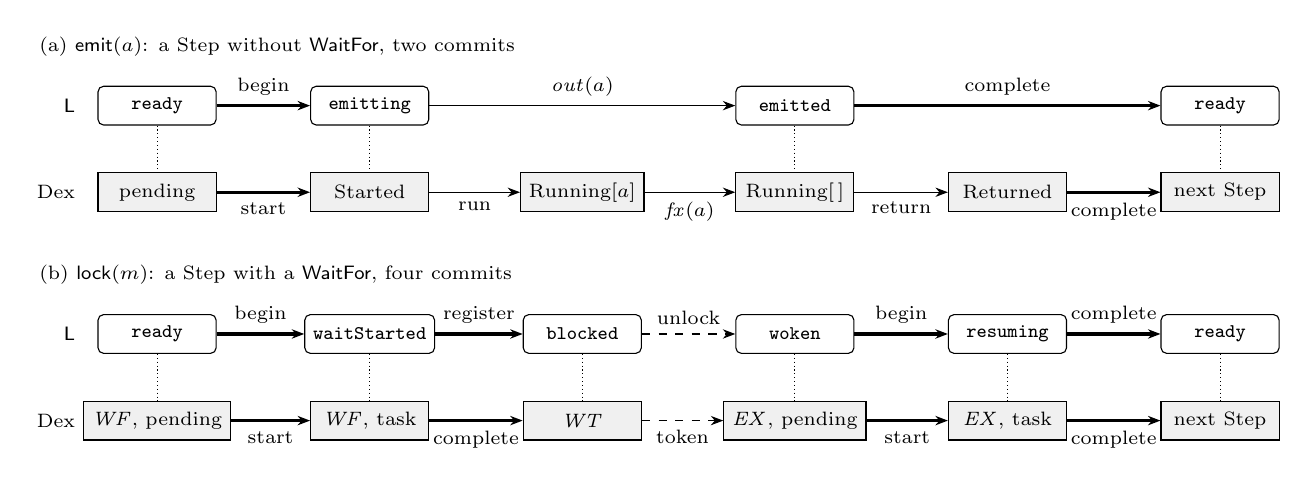
\begin{tikzpicture}[
  >={Stealth[length=4.5pt]},
  ph/.style={draw,rounded corners=2pt,font=\scriptsize\ttfamily,inner sep=3pt,minimum height=14pt,minimum width=1.5cm},
  dx/.style={draw,font=\scriptsize,inner sep=3pt,minimum height=14pt,minimum width=1.5cm,fill=black!6},
  lab/.style={font=\scriptsize},
  commit/.style={->,line width=1.1pt},
  other/.style={->},
  x=2.7cm,y=1cm]
% (a) emit
\node[lab,anchor=west] at (-0.6,3.75) {(a) \kw{emit}$(a)$: a Step without \kw{WaitFor}, two commits};
\node[lab,anchor=east] at (-0.34,3.0) {\Lang};
\node[ph] (l0) at (0,3.0) {ready};
\node[ph] (l1) at (1,3.0) {emitting};
\node[ph] (l2) at (3,3.0) {emitted};
\node[ph] (l3) at (5,3.0) {ready};
\draw[commit] (l0) -- node[lab,above] {begin} (l1);
\draw[other] (l1) -- node[lab,above] {$\mathit{out}(a)$} (l2);
\draw[commit] (l2) -- node[lab,above] {complete} (l3);
\node[lab,anchor=east] at (-0.34,1.9) {Dex};
\node[dx] (d0) at (0,1.9) {pending};
\node[dx] (d1) at (1,1.9) {Started};
\node[dx] (d2) at (2,1.9) {Running$[a]$};
\node[dx] (d3) at (3,1.9) {Running$[\,]$};
\node[dx] (d4) at (4,1.9) {Returned};
\node[dx] (d5) at (5,1.9) {next Step};
\draw[commit] (d0) -- node[lab,below] {start} (d1);
\draw[other] (d1) -- node[lab,below] {run} (d2);
\draw[other] (d2) -- node[lab,below] {$\mathit{fx}(a)$} (d3);
\draw[other] (d3) -- node[lab,below] {return} (d4);
\draw[commit] (d4) -- node[lab,below] {complete} (d5);
\foreach \a/\b in {l0/d0,l1/d1,l2/d3,l3/d5} \draw[densely dotted] (\a) -- (\b);
% (b) lock
\node[lab,anchor=west] at (-0.6,0.85) {(b) \kw{lock}$(m)$: a Step with a \kw{WaitFor}, four commits};
\node[lab,anchor=east] at (-0.34,0.1) {\Lang};
\node[ph] (b0) at (0,0.1) {ready};
\node[ph] (b1) at (1,0.1) {waitStarted};
\node[ph] (b2) at (2,0.1) {blocked};
\node[ph] (b3) at (3,0.1) {woken};
\node[ph] (b4) at (4,0.1) {resuming};
\node[ph] (b5) at (5,0.1) {ready};
\draw[commit] (b0) -- node[lab,above] {begin} (b1);
\draw[commit] (b1) -- node[lab,above] {register} (b2);
\draw[other,dashed] (b2) -- node[lab,above] {unlock} (b3);
\draw[commit] (b3) -- node[lab,above] {begin} (b4);
\draw[commit] (b4) -- node[lab,above] {complete} (b5);
\node[lab,anchor=east] at (-0.34,-1.0) {Dex};
\node[dx] (e0) at (0,-1.0) {$\mathit{WF}$, pending};
\node[dx] (e1) at (1,-1.0) {$\mathit{WF}$, task};
\node[dx] (e2) at (2,-1.0) {$\mathit{WT}$};
\node[dx] (e3) at (3,-1.0) {$\mathit{EX}$, pending};
\node[dx] (e4) at (4,-1.0) {$\mathit{EX}$, task};
\node[dx] (e5) at (5,-1.0) {next Step};
\draw[commit] (e0) -- node[lab,below] {start} (e1);
\draw[commit] (e1) -- node[lab,below] {complete} (e2);
\draw[other,dashed] (e2) -- node[lab,below] {token} (e3);
\draw[commit] (e3) -- node[lab,below] {start} (e4);
\draw[commit] (e4) -- node[lab,below] {complete} (e5);
\foreach \a/\b in {b0/e0,b1/e1,b2/e2,b3/e3,b4/e4,b5/e5} \draw[densely dotted] (\a) -- (\b);
\end{tikzpicture}
\caption{One \Lang{} statement and its Step. Upper lanes: the phases of the
thread (\lean{L.Phase}). Lower lanes: the Step's invocation and task. Thick
arrows are clock-stamped: a stamped \Lang{} action above, a Dex commit
(\rulename{STEP-START} or a Complete rule) below. (a) An \kw{emit} is
issued at \rulename{STEP-START}; $\ev{out}(a)$ is the Worker's effect; the
thread continues at \rulename{STEP-COMPLETE-EXECUTE}. The Worker's run and
return steps have no \Lang{} counterpart. (b) A blocked \kw{lock} is woken
by another thread's \kw{unlock} (dashed): the commit that publishes the
token moves the waiting Step from $\mathit{WT}$ to $\mathit{EX}$.}
\label{fig:lifecycle}
\end{figure}

\paragraph{The \kw{Execute} of a program point.}
\lean{pointStepDef} runs the thread-local semantics of the head statement
(\lean{L.completeStatement}, the same function \Lang{}'s own semantics
uses) and encodes the atomic action it asks for as Dex effects and a
decision (\lean{encodeIntent}). \lean{encodeIntent} is the mapping table of
the specification, one case per row; Table~\ref{tab:mapping} reproduces it.

\begin{table}[t]
\centering
\small
\begin{tabularx}{\textwidth}{@{}P{3.5cm}L@{}}
\toprule
\Lang{} construct & Dex mapping \\
\midrule
\kw{if}, \kw{while}, local assignment & A Step whose \kw{Execute} \kw{GoTo}s
  the next program point (the taken branch, the loop body, or the loop
  exit). \\
Shared read, shared write & One \kw{Execute} per access: read from the
  snapshot, or write one Attribute. \\
Call, \kw{return}, recursion & Push or pop a frame on the explicit stack in
  the Step input. No SubFlow. \\
\kw{throw}, \kw{try} & The handler stack is in the Step input; \kw{throw}
  is a \kw{GoTo} to the innermost handler's program point. No Worker
  error. \\
\kw{fork} & \kw{GoToMany}: the parent's continuation and the child's first
  program point. The child's thread ID is the parent's ID extended by the
  parent's counter. \\
Thread end & Publish one message to the Channel $\mathit{join}/t$, then
  \kw{DeadEnd}. \\
\kw{join}$(t)$ & \kw{WaitFor} returns
  $\kw{AnyOf}(\mathit{join}/t,\ \mathit{cancel}/\mathit{self})$. \\
\kw{exit}$(v)$, return of \kw{main} & \kw{ForceComplete} with the tagged
  value $\{\texttt{exit}: v\}$, which is never null. \\
\kw{fail}$(s)$, uncaught string exception & \kw{ForceFail}$(s)$. \\
Halted thread & \kw{DeadEnd}, publishing nothing. \\
\kw{newMutex}, \kw{unlock}$(m)$ & \kw{Execute} publishes one token to
  $m$'s token Channel. \\
\kw{lock}$(m)$ & \kw{WaitFor} returns $\kw{Until}(m\text{'s token})$, that
  is, \kw{AllOf} with one condition: a \kw{ForOne} waiter, FIFO by
  registration. \\
\kw{wait}$(\mathit{cv}, m)$ & Three Steps. (1) One \kw{Execute}, under $m$:
  append the thread ID $w$ to the Attribute $\mathit{waiters}/\mathit{cv}$
  and publish $m$'s token. (2) Wait on the per-waiter Channel
  $\mathit{cv}/w$. (3) \kw{lock}$(m)$ again. \\
\kw{signal}$(\mathit{cv})$ & One \kw{Execute}, under $m$: if
  $\mathit{waiters}/\mathit{cv}$ is not empty, remove its head $h$ and
  publish to $\mathit{cv}/h$. \\
\kw{broadcast}$(\mathit{cv})$ & As \kw{signal}, for every waiter in
  order. \\
\kw{cancel}$(t)$ & \kw{Execute} publishes to $\mathit{cancel}/t$. \\
\kw{recv}$(c)$ & \kw{WaitFor} returns
  $\kw{AnyOf}(c,\ \mathit{cancel}/\mathit{self})$. The environment's
  publications fill $c$. \\
\kw{sleep}$(d)$ & \kw{GoTo} the \lean{timed} Step (Enter). Its \kw{WaitFor}
  returns $\kw{AnyOf}(\mathit{Timer}(d),\ \mathit{cancel}/\mathit{self})$
  (Arm). \\
\kw{select} with \kw{after}$(d)$ & As \kw{sleep}, with the wait
  $\kw{AnyOf}(\mathit{Timer}(d),\ c,\ \mathit{cancel}/\mathit{self})$. Only
  the winner consumes. \\
\kw{emit}$(a)$ & An \kw{Execute} whose only external effect is $a$. \\
\bottomrule
\end{tabularx}
\caption{The translation, by construct (\lean{encodeIntent},
\lean{encodeWaitRequest}, \lean{timedStepDef} in
\file{Translation/Flow.lean}). Every Channel condition is \kw{ForOne}.}
\label{tab:mapping}
\end{table}

The translation uses \kw{GoTo}, \kw{GoToMany}, \kw{DeadEnd},
\kw{ForceComplete}, and \kw{ForceFail}, and nothing else: no
\kw{CancelSteps}, no \kw{GracefulComplete}, no RPCs, no SubFlows, no
Attribute locks. Every decision it returns is well formed for every input
(\lean{translate_execute_isWellFormed}).

\paragraph{Why the encodings are faithful.}
Each encoding rests on a property of the Dex core from
\S\ref{sec:dex-rules}.

\emph{Mutex.} A mutex is a Channel that holds one token exactly while the
mutex is unlocked. The Channel has only \kw{ForOne} waiters, so a wake
serves them in registration order, and a token that is present when a
waiter registers means that no earlier waiter was blocked. This gives
\Lang{}'s FIFO acquisition. An Attribute lock would not do: it is held for
one Step method, not across a wait.

\emph{Condition variable.} The waiter list is an Attribute. Reading and
writing it in one \kw{Execute} would normally be a lost-update hazard
(\S\ref{sec:dex-rules}); here it is safe because the \kw{Execute} runs
while its thread holds $m$, and no other thread touches the list. This is
where the mutex requirement enters: \Lang{} does not let a thread begin
such a statement without $m$, the translated Step has no such check, and
well-formedness says that the difference never shows. The wake goes to a
per-waiter Channel, so a signal reaches the dequeued waiter even if that
waiter has not registered its wait yet: the message stays queued. No
spurious wakeup is needed. The waiter list is an AttributeMap instance, so
the Step that reads it must select it in its load options; the model
applies the selection as the server does, and
\lean{readWaiters_snapshot_of_cvOperand} proves that the declared selection
is enough.

\emph{Cancellation.} A cancel is a message on the per-thread Channel
$\mathit{cancel}/t$. \kw{AnyOf} consumes only from the winning condition,
so a cancel never eats an input message or a join token. At registration no
timer is done, and the Channel conditions decide in declaration order, the
operation's own Channel before $\mathit{cancel}/\mathit{self}$. That is
\Lang{}'s rule that a cancel is observed only if the point would block. The
translation never cancels a Step. The only Step cancellation in a
translated Flow is the Flow close, after which nothing is observable except
effects already in flight, which \Lang{}'s asynchronous \kw{emit} allows.

\emph{Timers.} Every timed operation runs in the one Step type
\lean{timed}, with one timer at index 0. \Lang{}'s Enter is the commit that
creates the Step, so the timer number is the Step number. \Lang{}'s Arm is
the \kw{WaitFor} completion, so the deadline is the fire time. For equal
fire times Dex orders timers by encoded timer ID, which for these IDs is
numeric order on the Step number. A \rulename{TIMER-FIRE} prefix of size
$k$ is then $k$ consecutive \kw{fire} actions of \Lang{}.

\emph{Exit.} \kw{ForceComplete} drops a null output, so the translation
passes the tagged value $\{\texttt{exit}: v\}$, which is never null even
when $v$ is \Lang{}'s null. The projection reads $v$ back from the one
output of the closed Flow.

\section{The theorems}
\label{sec:theorems}

Both sides are instances of one structure,
\lean{TransitionSystem} (\file{Core/TransitionSystem.lean}): an initial
state, a partial step function that returns the events of a transition, the
request a label attempts (if any), whether a label is a \emph{progress
step}, and whether a state is \emph{closed}. Finite traces, runs for an
input word, markers, and fair maximal traces are defined once, for any
transition system, so the two trace sets of each statement are built the
same way. Figure~\ref{fig:overview} shows the shape of the claim.

\begin{figure}[t]
\centering
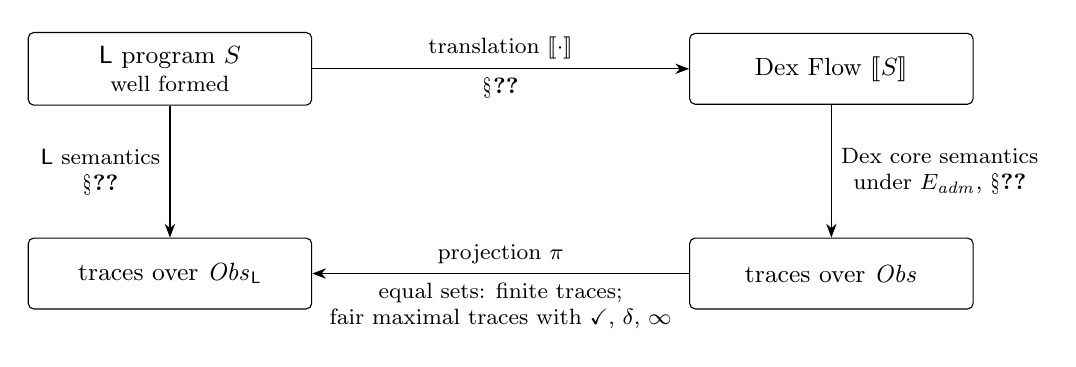
\begin{tikzpicture}[
  >={Stealth[length=5pt]},
  box/.style={draw,rounded corners=2pt,align=center,font=\small,inner sep=5pt,minimum width=3.6cm,minimum height=0.9cm},
  lab/.style={font=\footnotesize,align=center}]
\node[box] (S) at (0,2.6) {\Lang{} program $S$\\[-1pt]{\footnotesize well formed}};
\node[box] (F) at (8.4,2.6) {Dex Flow $\tr{S}$};
\node[box] (TL) at (0,0) {traces over \ObsL{}};
\node[box] (TD) at (8.4,0) {traces over \Obs{}};
\draw[->] (S) -- node[lab,above] {translation $\tr{\cdot}$} node[lab,below] {\S\ref{sec:translation}} (F);
\draw[->] (S) -- node[lab,left] {\Lang{} semantics\\ \S\ref{sec:language}} (TL);
\draw[->] (F) -- node[lab,right] {Dex core semantics\\ under \Eadm{}, \S\ref{sec:dex}} (TD);
\draw[->] (TD) -- node[lab,above] {projection $\pi$} node[lab,below] {equal sets: finite traces;\\ fair maximal traces with \mterm, \mdead, \mdiv} (TL);
\end{tikzpicture}
\caption{The claim. The traces of the translated Flow, projected to
\Lang{}'s alphabet, are the traces of the program.}
\label{fig:overview}
\end{figure}

\subsection{The admissible environment and the projection}

The Dex alphabet has raw identifiers and the theorem's environment is
restricted, so the statement is over a projection, under an admissible
environment.

\paragraph{\Eadm.}
An admissible input word is a finite or infinite sequence of
\emph{attempted} client requests, accepted and rejected alike. It begins
with exactly one request that starts the Flow at the entry Step with the
program input. Every later request publishes one message to one of the
program's external Channels. The start input and every message are encoded
\Lang{} literals (\S\ref{sec:scope}). There is no other client operation.
In Lean, \lean{Translation.environment} fixes these data and
\lean{Dex.Environment.IsAdmissibleWord} states the shape. The \Lang{} form
is \lean{L.IsAdmissibleWord}: one \lean{start}, then \lean{input} requests.
The lemmas \lean{isAdmissibleWord_encode} and \lean{isAdmissibleWord_decode}
show that the encoded admissible \Lang{} words are exactly the words of
\Eadm.

Counting attempted requests, and not only accepted ones, matters. A
publication after the Flow closed is rejected and produces only a
$\ev{rejected}$ event; \Lang{} produces $\ev{refused}$ for the same input.
A word of accepted events only would give the \Lang{} run that exits and
then refuses an input no matching Dex run.

\paragraph{$\pi$.}
The projection $\pi : \Obs \to \ObsL \cup \{\varepsilon\}$
(\lean{Translation.project}) is given by Table~\ref{tab:projection}.

\begin{table}[t]
\centering
\small
\begin{tabular}{@{}ll@{}}
\toprule
Dex event & \Lang{} event \\
\midrule
$\ev{start}(T_0, \mathit{enc}(v))$ & $\ev{begin}(v)$ \\
$\ev{pub}(c, \mathit{enc}(v))$, $c$ external & $\ev{in}(c, v)$ \\
$\ev{rejected}(\ev{pub}(c, \mathit{enc}(v)))$, $c$ external & $\ev{refused}(c, v)$ \\
$\ev{fx}(e, m, a)$ & $\ev{out}(a)$ \quad (the source is dropped) \\
$\ev{closed}(\mathit{Completed}, [(e, \{\texttt{exit}: v\})])$ & $\ev{exit}(v)$ \\
$\ev{closed}(\mathit{Failed}(s), \_)$ & $\ev{fail}(s)$ \\
every other event & $\varepsilon$ \\
\bottomrule
\end{tabular}
\caption{The projection $\pi$ from Dex events to \Lang{} events.}
\label{tab:projection}
\end{table}

\subsection{Safety}

A finite trace of a system is the event sequence of a finite run from the
initial state, viewed through a function that may erase events
(\lean{TransitionSystem.IsFiniteTrace}). The two sets of
Equation~\eqref{eq:safety} are (\file{TraceSets.lean}):

\begin{Verbatim}
def IsProjectedDexFiniteTrace (program : Program) (trace : List Event) : Prop :=
  (Dex.system ⟦program⟧).IsFiniteTrace environment.IsAdmissiblePrefix project trace

def IsLFiniteTrace (program : Program) (trace : List Event) : Prop :=
  (L.system program).IsFiniteTrace (fun _ => True) some trace
\end{Verbatim}

Lean's core library has no set type, so an equality of sets is written as a
bi-implication for every element. The safety theorem
(\file{Theorems.lean}) is:

\begin{Verbatim}
theorem safety_of_isWellFormed (program : Program) (isWellFormed : program.IsWellFormed)
    (trace : List Event) :
    IsProjectedDexFiniteTrace program trace ↔ IsLFiniteTrace program trace
\end{Verbatim}

This is weak trace equality: Dex transitions without a projected event are
invisible. Finite traces alone cannot tell a Flow whose last thread ended
with \kw{DeadEnd}, and which stays running forever, from a Flow whose close
an unfair scheduler never runs. Liveness closes that gap.

\subsection{Liveness}
\label{sec:liveness-statement}

\paragraph{Runs for a word.}
Clock ticks are always enabled, so no maximal run is finite. A run
\emph{for} an input word $w$ is an infinite run whose request transitions
are exactly the requests of $w$, each once and in order
(\lean{IsRunFor}). A tick is time passing, not progress; every other
transition is a progress step.

\paragraph{Fairness.}
The rules themselves are unfair: the dispatcher may delay a startable
method, the timer service a due timer, and a Worker its response, each
without bound. Liveness is therefore stated for fair runs. The conditions
are assumptions about the scheduler, the timer service, and the Workers.
They are not guarantees that the rules provide. Table~\ref{tab:fairness}
states them on both sides. Each of F2 to F5 is a weak-fairness condition of
one shape (\lean{EventuallyFails}): a given predicate on the state does not
hold forever from any point on.

\begin{table}[t]
\centering
\small
\begin{tabularx}{\textwidth}{@{}P{0.6cm}LL@{}}
\toprule
 & Dex (\lean{Dex.IsFair}, \file{Dex/Observation.lean}) &
   \Lang{} (\lean{L.IsFair}, \file{L/Semantics.lean}) \\
\midrule
F0 & Every request of $w$ is eventually attempted, in order. It follows
  from ``run for $w$''. & The same. \\
F1 & The clock exceeds every bound. & The same. \\
F2 & No timer stays armed and due forever. An assumption on the timer
  service: it eventually proposes \rulename{TIMER-FIRE}. & No thread's
  armed timer stays due forever: \kw{fire} eventually happens. \\
F3 & No invocation stays pending forever. An assumption on dispatch: a
  pending method is eventually handed to a Worker. In this fragment every
  pending invocation is startable, because there are no locks. & No thread
  stays forever in a phase in which its next action has not begun
  (\lean{bootPending}, \lean{ready}, \lean{woken}). \\
F4 & No task stays in $\Theta$ forever without having returned: it emits
  all its effects and returns, or, if its invocation was canceled, it is
  dropped after some prefix of its effects. An assumption on the Workers:
  handlers terminate, and a Worker whose task was canceled eventually stops
  or finishes. & No thread stays \lean{emitting} forever while the program
  runs; after the end, a non-empty list of late emits eventually
  shrinks. \\
F5 & No task stays \emph{Returned} forever: its result commits, or it is
  dropped as stale. An assumption on the engine: a returned response is
  eventually proposed as a commit. & No thread stays forever in a phase in
  which it began an action and has not completed it. \\
F6 & Cross-Flow messages are delivered. Vacuous here: one Flow. &
  Vacuous. \\
\bottomrule
\end{tabularx}
\caption{The fairness assumptions. They constrain runs; no rule enforces
them.}
\label{tab:fairness}
\end{table}

F4 deserves emphasis. The server does not make a Worker finish. It hands a
method to a Worker, and for a canceled method it sends a cancel request;
cancellation is cooperative. That every task eventually leaves $\Theta$ is
an assumption about Workers that run terminating handlers and honor
cancellation or run to completion. A Worker that hangs forever on a task
gives an unfair run, about which the theorem says nothing.

\paragraph{Markers.}
A fair run is infinite, because time keeps passing. It is classified by its
progress steps (\lean{HasMarker}):
\begin{itemize}
\item \mterm{} (\lean{terminated}): finitely many progress steps, and the
  program is closed at some point.
\item \mdead{} (\lean{deadlocked}): finitely many progress steps, and the
  program is never closed. From some point on only ticks happen: nothing
  can start, no task is in flight, no timer is armed, and the word is used
  up. A program whose threads all ended without \kw{exit} lands here.
\item \mdiv{} (\lean{divergent}): infinitely many progress steps.
\end{itemize}
A \mterm{} run has finitely many progress steps, so by F4 and F5 no task
is left in $\Theta$ after the last one. The trace therefore already contains
every effect that a canceled Worker emits after the close, and a \mterm{}
trace is never a proper prefix of another fair trace for the same word.

\paragraph{The statement.}
A fair maximal trace for $w$ is the whole observable trace of a fair run
for $w$, with the run's marker (\lean{IsFairMaximalTrace}). The two sets of
Equation~\eqref{eq:liveness} are:

\begin{Verbatim}
def IsProjectedDexFairMaximalTrace (program : Program) (word : Sequence L.Request)
    (trace : Sequence Event) (marker : Marker) : Prop :=
  (Dex.system ⟦program⟧).IsFairMaximalTrace Dex.IsFair project
    (word.map encodeRequest) trace marker

def IsLFairMaximalTrace (program : Program) (word : Sequence L.Request)
    (trace : Sequence Event) (marker : Marker) : Prop :=
  (L.system program).IsFairMaximalTrace L.IsFair some word trace marker
\end{Verbatim}

A \lean{Sequence} is a finite or infinite sequence. The word is quantified
in \Lang{} form and encoded for the Dex side. The liveness theorem is:

\begin{Verbatim}
theorem liveness_of_isWellFormed (program : Program) (isWellFormed : program.IsWellFormed)
    (word : Sequence L.Request) (isAdmissible : L.IsAdmissibleWord word)
    (trace : Sequence Event) (marker : Marker) :
    IsProjectedDexFairMaximalTrace program word trace marker ↔
      IsLFairMaximalTrace program word trace marker
\end{Verbatim}

\lean{expressiveness_of_isWellFormed} is the conjunction of the two
theorems. The theorem names carry the scope, so that it is visible wherever
a theorem is used.

\paragraph{Why this equivalence.}
The specification chose trace equality over weak bisimilarity, which is
stronger than the claim needs and distinguishes \emph{where} a
nondeterministic choice is made. Trace equality with markers, per input
word, still separates normal exit, failure, deadlock, and divergence, and
it accounts for effects after the close. The proof does establish step
simulations in both directions over one relation (\S\ref{sec:proof}); the
theorems state only what follows for traces. The theorem is untimed: clock values are not observable. Time still
matters, through the order in which timers fire and through F1 and F2.

\paragraph{What the kernel checked.}
For both theorems, \texttt{\#print axioms} reports
\lean{propext}, \lean{Classical.choice}, and \lean{Quot.sound}: the three
standard axioms of Lean, and nothing else. No file contains \texttt{sorry},
and the proofs do not use \lean{native_decide}. The trusted base is the
Lean~4 kernel \cite{demoura2021lean4} and the definitions a reader must
check against the specification: the transition-system core, the Dex model,
the \Lang{} model, the translation, the projection, and the two statements,
about 3,450 lines in 14 files.

\section{The proof}
\label{sec:proof}

The proof has the classical shape of a simulation argument
\cite{lynch1995simulations,abadi1991refinement}: a relation between the
states of the two systems, invariants of each side, a step simulation in
each direction, and then the lifting of those steps to finite and infinite
runs. Figure~\ref{fig:architecture} shows the parts. This section describes
them in order and says where each one is in the Lean development.

\begin{figure}[t]
\centering
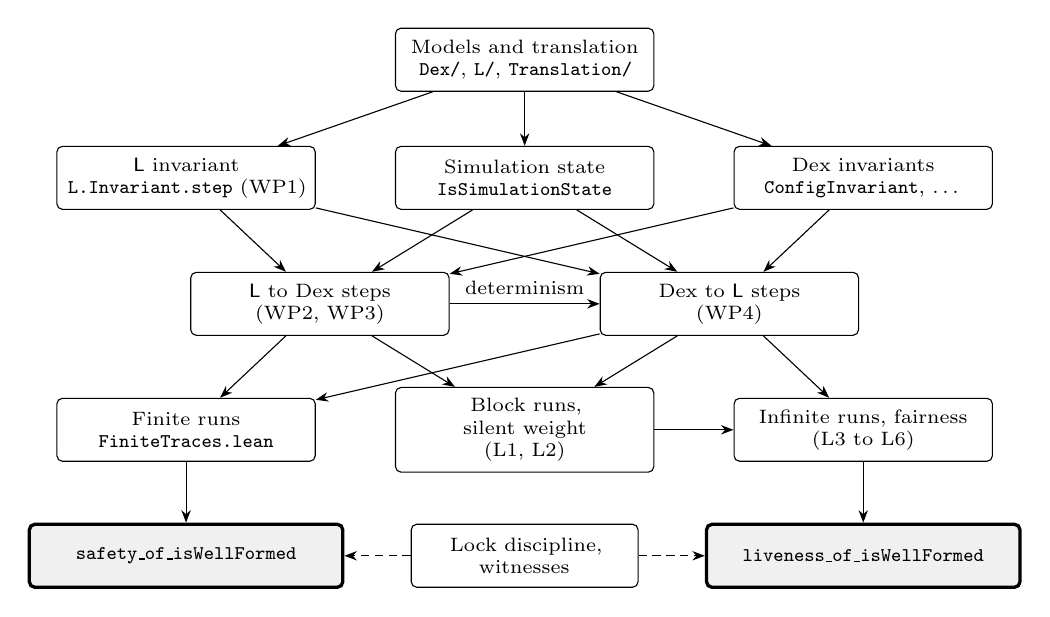
\begin{tikzpicture}[
  >={Stealth[length=4.5pt]},
  box/.style={draw,rounded corners=2pt,align=center,font=\scriptsize,inner sep=4pt,minimum height=0.8cm,text width=3.0cm},
  thm/.style={box,very thick,fill=black!6,text width=3.7cm},
  x=1cm,y=1cm]
\node[box] (model) at (0,5.4) {Models and translation\\ \texttt{Dex/}, \texttt{L/}, \texttt{Translation/}};
\node[box] (linv) at (-4.3,3.9) {\Lang{} invariant\\ \texttt{L.Invariant.step} (WP1)};
\node[box] (rel) at (0,3.9) {Simulation state\\ \texttt{IsSimulationState}};
\node[box] (dinv) at (4.3,3.9) {Dex invariants\\ \texttt{ConfigInvariant}, \ldots};
\node[box] (ltod) at (-2.6,2.3) {\Lang{} to Dex steps\\ (WP2, WP3)};
\node[box] (dtol) at (2.6,2.3) {Dex to \Lang{} steps\\ (WP4)};
\node[box] (fin) at (-4.3,0.7) {Finite runs\\ \texttt{FiniteTraces.lean}};
\node[box] (blocks) at (0,0.7) {Block runs, silent weight\\ (L1, L2)};
\node[box] (inf) at (4.3,0.7) {Infinite runs, fairness\\ (L3 to L6)};
\node[thm] (safety) at (-4.3,-0.9) {\texttt{safety\_of\_isWellFormed}};
\node[thm] (live) at (4.3,-0.9) {\texttt{liveness\_of\_isWellFormed}};
\node[box,text width=2.6cm] (disc) at (0,-0.9) {Lock discipline,\\ witnesses};
\draw[->] (model) -- (linv);
\draw[->] (model) -- (rel);
\draw[->] (model) -- (dinv);
\draw[->] (linv) -- (ltod);
\draw[->] (rel) -- (ltod);
\draw[->] (rel) -- (dtol);
\draw[->] (dinv) -- (dtol);
\draw[->] (dinv) -- (ltod);
\draw[->] (linv) -- (dtol);
\draw[->] (ltod) -- node[font=\scriptsize,above] {determinism} (dtol);
\draw[->] (ltod) -- (fin);
\draw[->] (dtol) -- (fin);
\draw[->] (ltod) -- (blocks);
\draw[->] (dtol) -- (blocks);
\draw[->] (blocks) -- (inf);
\draw[->] (dtol) -- (inf);
\draw[->] (fin) -- (safety);
\draw[->] (inf) -- (live);
\draw[->,densely dashed] (disc) -- (safety);
\draw[->,densely dashed] (disc) -- (live);
\end{tikzpicture}
\caption{The structure of the proof. WP1 to WP4 are the work packages of
safety, L1 to L6 those of liveness (\S\ref{sec:engineering}). The dashed
arrows are non-vacuity (\S\ref{sec:nonvacuity}): the hypothesis holds for
concrete programs, and the trace sets are inhabited.}
\label{fig:architecture}
\end{figure}

\subsection{The simulation state}
\label{sec:relation}

Every step lemma takes one hypothesis, \lean{IsSimulationState}
(\file{Simulation/Relation.lean}), with five parts:

\begin{Verbatim}
structure IsSimulationState (program : Program) (lConfig : L.Config)
    (dexConfig : Dex.Config signature) : Prop where
  isRelated : Related program lConfig dexConfig
  lInvariant : L.Invariant program lConfig
  dexInvariant : ConfigInvariant program dexConfig
  tasksDistinct : TasksAreDistinct dexConfig
  timersDistinct : TimersAreDistinct dexConfig
\end{Verbatim}

\paragraph{\lean{Related}} holds only the clauses that mention both sides.
The clocks agree, and the last stamped \Lang{} action carries the timestamp
of the last Dex commit: this is the timing model at work. The statuses
correspond (not started, running, closed). While the program runs
(\lean{RunningRelated}):
\begin{itemize}
\item \emph{Data.} Shared variables are Attributes; each condition
  variable's queue is its waiter-list Attribute; each external channel's
  queue is its Channel's pending messages.
\item \emph{Tokens.} A mutex's token Channel holds one token exactly while
  the mutex is unlocked; $\mathit{join}/t$ holds one message exactly while
  $t$ has ended and was not joined; $\mathit{cv}/w$ holds the wakes of a
  waiter that has not parked yet. A pending cancel request means the flag
  is set; a set flag means a pending request, or a thread that has observed
  it, or an ended thread that no live thread can still fork.
\item \emph{Timers.} The armed Dex timers are the armed \Lang{} timers,
  with the same number and deadline, and the timer counter is the counter
  of the \lean{timed} Step type.
\item \emph{Threads and Steps.} Every thread that has not halted is carried
  by exactly one active Step, and every active Step carries one thread
  (\lean{StepCarriesThread}): the Step has the type, input, and options the
  translation gives that thread. The thread's phase fixes the Step's phase,
  invocation, and task (\lean{PhaseMatchesStep}), as in
  Figure~\ref{fig:lifecycle}. In particular a Step is in phase
  $\mathit{WT}$ exactly while its thread is blocked, so a publication wakes
  a Step exactly when it wakes the thread.
\item \emph{Order.} Two blocked threads are ordered by their blocking
  stamps as their Steps' waits are ordered by $\mathit{sws}$. This carries
  FIFO from one side to the other.
\end{itemize}
After the close (\lean{ClosedRelated}), the late emits of \Lang{} are, up to
permutation, the effects that the remaining stale tasks have not emitted
yet; no Step has an invocation, and no timer is armed.

\paragraph{The invariants.}
\lean{L.Invariant} (\file{L/Invariant.lean}) holds the facts about \Lang{}
alone: thread IDs are unique and the next children of a thread are fresh;
the next mutex a thread creates does not exist yet; every handle to a
\emph{created} mutex, or to a condition variable of one, that a thread
can reach names a mutex that \kw{newMutex} has created (this is where
unforgeable handles are used);
blocking stamps and timer numbers are distinct; each thread's phase
fits its code; a thread that began a statement that requires a mutex holds
it until the statement completes. The invariant does not check a static
index against the program's number of static mutexes:
\kw{staticMutex}$(i)$ with $i$ out of range names a mutex that never
exists, and a \kw{lock} of it blocks forever on both sides. On the Dex
side,
\lean{ConfigInvariant} wraps a run invariant (\lean{Dex.Run.Invariant}:
unique Step IDs, counted Step numbers, injective $\mathit{sws}$, only the
wait shapes the translation uses, and no pending message on a Channel that
a waiting Step names) and says that a task holds the response its handler
computes; \lean{TasksAreDistinct} and \lean{TimersAreDistinct} say
that task IDs and armed timer IDs are unique. Each invariant is proved to
hold initially and to be kept by every transition
(\lean{L.Invariant.step}, \lean{ConfigInvariant.step},
\lean{TasksAreDistinct.step}, \lean{TimersAreDistinct.step}).

\subsection{From \Lang{} to Dex: named action sequences}
\label{sec:ltodex}

The \Lang{}-to-Dex direction does not say ``there exist Dex actions''. It
names them. \lean{simulatingActions} is a function of the two
configurations and the \Lang{} label:

\begin{itemize}
\item a tick, a request, and a batch of \kw{fire} actions are one Dex action
  each (\lean{tick}, \lean{request}, \lean{timerFire});
\item a thread that begins an action is the \rulename{STEP-START} of its
  Step;
\item $\ev{out}(a)$ is the \lean{workerEffect} of the thread's task, after
  the \lean{workerRun} that runs the handler if it has not run;
\item a thread that completes an action is the \lean{stepComplete} of its
  task, after the \lean{workerRun} and \lean{workerReturn} that have not
  happened yet;
\item after the close, the delivery or the drop of a late emit is the
  \lean{workerEffect} or the \lean{workerAbandon} of the first task that
  still holds the effect.
\end{itemize}
So one \Lang{} label is one to three Dex actions. The step lemma, proved by
cases on the label (\lean{l_step_simulatedByActions},
\file{Simulation/LToDex.lean}), says that these actions are enabled, have
the same projected events, and end in a related configuration:

\begin{Verbatim}
def IsSimulatedByActions (program : Program) (lConfig : L.Config)
    (dexConfig : Dex.Config signature) (label : L.Label) (lEvents : List Event)
    (lNext : L.Config) : Prop :=
  ∃ dexEvents dexNext,
    (Dex.system ⟦program⟧).exec dexConfig (simulatingActions program lConfig dexConfig label) =
      some (dexEvents, dexNext) ∧
    dexEvents.filterMap project = lEvents ∧
    Related program lNext dexNext
\end{Verbatim}

The bulk of the proof is here. Registering a wait
(\file{Simulation/Register.lean}) and completing an action
(\file{Simulation/Completion.lean} and \file{Simulation/Completion/}) must
re-establish every clause of \lean{Related} after a commit that may write
an Attribute, publish tokens, wake the earliest waiter, create Steps, or
close the Flow.

\subsection{From Dex to \Lang{}: at most one label, by determinism}
\label{sec:dextol}

In the other direction, every Dex step of an admissible run is simulated by
at most one \Lang{} label (\lean{dex_step_simulated},
\file{Simulation/DexToL.lean}):

\begin{Verbatim}
def IsSimulatedByL (program : Program) (lConfig : L.Config)
    (dexEvents : List (Dex.Obs signature)) (dexNext : Dex.Config signature) : Prop :=
  ∃ labels lNext,
    labels.length ≤ 1 ∧
    (L.system program).exec lConfig labels = some (dexEvents.filterMap project, lNext) ∧
    Related program lNext dexNext
\end{Verbatim}

Running a handler, returning it, and dropping a task that holds no effect
have no \Lang{} label: the list is empty and the relation is kept. For the
actions that \Lang{} sees, the proof does not repeat the case analysis of
the relation. It reuses the other direction:
\begin{enumerate}
\item Show that the corresponding \Lang{} label is enabled.
\item Apply the \Lang{}-to-Dex lemma. It names the simulating Dex actions.
\item Show that those actions are the given action alone. For a Worker
  effect or a completion, the given action is enabled only when the Worker
  steps before it have already happened, so the named list has no prefix.
\item \lean{Dex.step} is a function. The given step is therefore the
  simulating step, and its result is the related configuration of step 2.
\end{enumerate}
This is why the \Lang{}-to-Dex statement names its actions: an existential
statement could not be matched against a given Dex step. Compiler
verification uses determinism for a similar economy: with a deterministic
target, preservation proved in one direction suffices
\cite{leroy2009compcert}.

Step~1 is the only place where well-formedness is used. At
\rulename{STEP-START} of a Step whose statement requires a mutex, the
\Lang{} thread can begin only if it holds the mutex; the hypothesis that
\lean{BreaksMutexRequirement} does not hold says that it does. Consequently the
two \Lang{}-to-Dex inclusions, \lean{finiteTrace_l_to_dex} and
\lean{fairMaximalTrace_l_to_dex}, hold for every program; only the
Dex-to-\Lang{} inclusions need the scope.

\subsection{Safety}

Safety follows by induction on a finite run
(\file{FiniteTraces.lean}). The initial configurations are a simulation
state (\lean{related_initial} and the initial cases of the invariants). Each
step of one side is matched by the step simulation, and the invariants are
carried along by their own step lemmas. The Dex-to-\Lang{} induction also
carries reachability of the \Lang{} configuration, to apply
well-formedness, and admissibility of each Dex action, which follows from
the admissible prefix. The two inclusions are \lean{finiteTrace_dex_to_l}
and \lean{finiteTrace_l_to_dex}.

\subsection{Liveness}
\label{sec:liveness-proof}

Each inclusion of liveness builds an infinite run of one side from an
infinite run of the other, and then carries over the input word, the trace,
the marker, and the fairness assumptions.

\paragraph{Runs in blocks.}
The two systems do not step in lockstep. One \Lang{} label is one to three
Dex actions, and a Dex Worker step is no \Lang{} label. A run of one side
therefore gives the other side a \emph{run in blocks}
(\lean{BlockRun}, \file{Core/BlockRun.lean}): one finite, possibly empty,
list of labels per step of the first (Figure~\ref{fig:blocks}). A block run
with infinitely many non-empty blocks \emph{flattens} into an ordinary
infinite run (\lean{BlockRun.IsFlattenedTo}), and the flattening keeps the
trace, the attempted requests, and whether the progress steps are finitely
many. This part mentions neither Dex nor \Lang{}.

\begin{figure}[t]
\centering
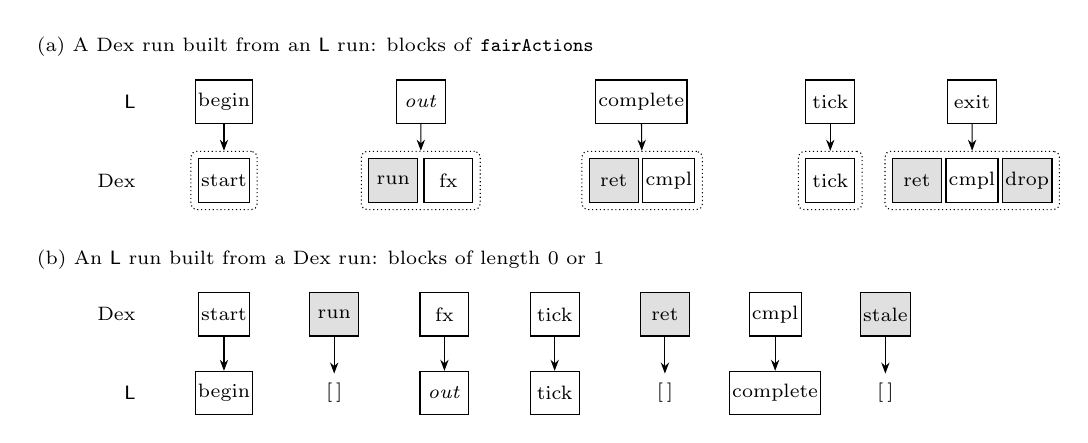
\begin{tikzpicture}[
  >={Stealth[length=4pt]},
  cell/.style={draw,minimum height=0.55cm,minimum width=0.62cm,font=\scriptsize,inner sep=1pt},
  sil/.style={cell,fill=black!12},
  lab/.style={font=\scriptsize},
  blk/.style={draw,densely dotted,rounded corners=2pt,inner sep=2.5pt},
  x=1cm,y=1cm]
% (a) L run -> Dex blocks
\node[lab,anchor=west] at (-1.6,2.9) {(a) A Dex run built from an \Lang{} run: blocks of \texttt{fairActions}};
\node[lab,anchor=east] at (-0.1,2.2) {\Lang{}};
\node[cell] (a0) at (0.9,2.2) {begin};
\node[cell] (a1) at (3.4,2.2) {$\mathit{out}$};
\node[cell] (a2) at (6.2,2.2) {complete};
\node[cell] (a3) at (8.6,2.2) {tick};
\node[cell] (a4) at (10.4,2.2) {exit};
\node[lab,anchor=east] at (-0.1,1.2) {Dex};
\node[cell] (p0) at (0.9,1.2) {start};
\node[sil] (p1) at (3.05,1.2) {run};
\node[cell] (p2) at (3.75,1.2) {fx};
\node[sil] (p3) at (5.85,1.2) {ret};
\node[cell] (p4) at (6.55,1.2) {cmpl};
\node[cell] (p5) at (8.6,1.2) {tick};
\node[sil] (p6) at (9.7,1.2) {ret};
\node[cell] (p7) at (10.4,1.2) {cmpl};
\node[sil] (p8) at (11.1,1.2) {drop};
\node[blk,fit=(p0)] (g0) {};
\node[blk,fit=(p1)(p2)] (g1) {};
\node[blk,fit=(p3)(p4)] (g2) {};
\node[blk,fit=(p5)] (g3) {};
\node[blk,fit=(p6)(p7)(p8)] (g4) {};
\draw[->] (a0) -- (g0);
\draw[->] (a1) -- (g1);
\draw[->] (a2) -- (g2);
\draw[->] (a3) -- (g3);
\draw[->] (a4) -- (g4);
% (b) Dex run -> L blocks
\node[lab,anchor=west] at (-1.6,0.2) {(b) An \Lang{} run built from a Dex run: blocks of length 0 or 1};
\node[lab,anchor=east] at (-0.1,-0.5) {Dex};
\node[cell] (q0) at (0.9,-0.5) {start};
\node[sil] (q1) at (2.3,-0.5) {run};
\node[cell] (q2) at (3.7,-0.5) {fx};
\node[cell] (q3) at (5.1,-0.5) {tick};
\node[sil] (q4) at (6.5,-0.5) {ret};
\node[cell] (q5) at (7.9,-0.5) {cmpl};
\node[sil] (q6) at (9.3,-0.5) {stale};
\node[lab,anchor=east] at (-0.1,-1.5) {\Lang{}};
\node[cell] (r0) at (0.9,-1.5) {begin};
\node[lab] (r1) at (2.3,-1.5) {$[\,]$};
\node[cell] (r2) at (3.7,-1.5) {$\mathit{out}$};
\node[cell] (r3) at (5.1,-1.5) {tick};
\node[lab] (r4) at (6.5,-1.5) {$[\,]$};
\node[cell] (r5) at (7.9,-1.5) {complete};
\node[lab] (r6) at (9.3,-1.5) {$[\,]$};
\foreach \a/\b in {q0/r0,q1/r1,q2/r2,q3/r3,q4/r4,q5/r5,q6/r6} \draw[->] (\a) -- (\b);
\end{tikzpicture}
\caption{Runs in blocks. Dotted outlines are blocks. Shaded Dex actions are
of a \emph{silent kind}:
\Lang{} has no label for them. (a) Each \Lang{} label becomes its
simulating actions, followed, after the close, by the drops of the canceled
tasks that hold no effect. (b) Each Dex action becomes at most one \Lang{}
label; silent actions become empty blocks.}
\label{fig:blocks}
\end{figure}

\paragraph{Dex to \Lang{}: the silent weight.}
Given a fair Dex run, \lean{dex_step_simulated} gives an \Lang{} run in
blocks of length 0 or 1 (\lean{LFollowsDex}). The danger is an infinite
tail of empty blocks: the Dex run would have infinitely many progress steps
(\mdiv) while the \Lang{} run has finitely many. The proof rules it out
with a measure. The actions that can have no \Lang{} label are of four
kinds: \lean{workerRun}, \lean{workerReturn}, \lean{workerAbandon}, and
\lean{stepCompleteStale}. A task can take at most three such steps (run,
return, drop), and the \emph{silent weight} of a configuration counts what
is left:

\begin{Verbatim}
def Dex.Task.silentWeight {σ : Dex.Signature} (task : Dex.Task σ) : Nat :=
  match task.phase with
  | .started => 3
  | .running _ _ => 2
  | .returned _ => 1

def Dex.Config.silentWeight {σ : Dex.Signature} (config : Dex.Config σ) : Nat :=
  (config.tasks.map Dex.Task.silentWeight).sum
\end{Verbatim}

Every action of a silent kind strictly lowers the weight
(\lean{silentWeight_lt_of_isSilentKind}), a tick keeps it, and only a step
that \Lang{} sees can raise it. So infinitely many progress steps of the
Flow include infinitely many that \Lang{} sees, and the \Lang{} labels of a
Dex step are progress steps exactly when the action is one. The markers
then agree. F1 gives infinitely many ticks, hence infinitely many non-empty
blocks, so the flattening exists (\lean{exists_lRun_of_dexRun}).

\paragraph{\Lang{} to Dex: cleaning up after the close.}
Given a fair \Lang{} run, the simulating actions give a Dex run in blocks
(\lean{DexFollowsL}). One more step is needed for fairness. When the
program ends, the Flow close cancels every active Step, and the tasks of
those Steps stay in $\Theta$. A stale task that still holds an effect
corresponds to a late emit, and \Lang{}'s own fairness delivers or drops
it. A stale task that holds no effect has no \Lang{} step at all, yet F4
requires it to leave $\Theta$. So the Dex run does not use
\lean{simulatingActions} alone. It uses \lean{fairActions}: the simulating
actions, followed by the \rulename{WORKER-ABANDON} of every canceled task
that holds no effect (\lean{cleanupActions}). Between two blocks no such
task and no \emph{Returned} task is left.

\paragraph{Fairness and markers carry over.}
For each direction, one lemma per assumption shows that the built run is
fair when the given run is. The correspondences are those of
Table~\ref{tab:fairness}: a thread whose next action has not begun is a
pending invocation (F3); a thread that issued an emit or began an action is
a task, with an effect exactly when it issued an emit (F4, F5); a due timer
is a due timer (F2); a late emit is an effect of a stale task (F4). The
markers carry over because closed corresponds to closed in \lean{Related}
and because flattening keeps whether the progress steps are finitely many.
The two inclusions are \lean{fairMaximalTrace_dex_to_l} and
\lean{fairMaximalTrace_l_to_dex} (\file{Liveness.lean}).

\subsection{Non-vacuity}
\label{sec:nonvacuity}

A theorem with a hypothesis is only as good as the set of objects that
satisfy the hypothesis. \lean{Program.IsWellFormed} quantifies over every
reachable configuration, so a concrete trace does not establish it, and
without a witness the theorems could hold for no program at all.

\paragraph{A static lock discipline.}
\file{L/LockDiscipline.lean} defines a decidable, syntactic, sufficient
condition, \lean{Program.hasStaticLockDiscipline}: a must-hold lock-set
analysis over the statically known mutexes.
\kw{lock}$(\kw{staticMutex}(i))$ adds $i$ to the set. \kw{unlock},
\kw{wait}, \kw{signal}, and \kw{broadcast} need a statically known operand
whose mutex is in the set. The two branches of an \kw{if} or a \kw{select}
must agree. A loop body must give back the set it started with. A called or
forked procedure body, a \kw{try} body, and a handler are checked from the
empty set. \file{L/LockDisciplineSound.lean} proves soundness:

\begin{Verbatim}
theorem Program.isWellFormed_of_hasStaticLockDiscipline (program : Program)
    (isDisciplined : program.hasStaticLockDiscipline = true) : program.IsWellFormed
\end{Verbatim}

The proof rests on one fact of \Lang{}: only the owner of a mutex releases
it, so the steps of other threads never shrink the set of mutexes a thread
holds.

\paragraph{Well-formed programs exist.}
\file{Examples/WellFormed.lean} proves \lean{IsWellFormed} for eight
programs, each by evaluating the discipline in the Lean kernel. Together
they use every construct of \Lang{}: a two-thread mutex program; a program
with \kw{sleep}, a timed \kw{select}, \kw{recv}, \kw{cancel}, \kw{fork},
and \kw{join}; a \kw{wait}/\kw{signal} program; a
\kw{wait}-in-a-loop/\kw{broadcast} program with shared variables; a
recursive program; a program with \kw{try}, a \kw{throw} across a call, and
an uncaught exception; three threads racing in \kw{select}; and a program
that creates and locks a mutex and then fails.
\file{Examples/WellFormedSafety.lean} states the safety theorem at three of
them with no hypothesis left, for example:

\begin{Verbatim}
theorem mutexProgram_safety (trace : List Event) :
    IsProjectedDexFiniteTrace Mutex.program trace ↔ IsLFiniteTrace Mutex.program trace :=
  safety_of_isWellFormed Mutex.program mutexProgram_isWellFormed trace
\end{Verbatim}

The trace sets are not empty either. \file{Examples/Mutex.lean} shows, by
running explicit schedules in the kernel, that both complete traces of the
two-thread mutex program are finite traces of the program and projected
finite traces of its Flow (\lean{bothTraces_onBothSides}).
\file{Examples/TimedSelect.lean} and \file{Examples/TimerOrder.lean} do the
same for timers, \kw{select}, cancellation, and two timers with equal
deadlines.

\paragraph{Fair maximal traces exist.}
The trace sets of liveness are defined by the existence of a fair run.
Without a fair run of some program, \lean{liveness_of_isWellFormed} would
compare two empty sets. \file{Liveness/RestingRuns.lean} builds fair
maximal runs of \Lang{}. A configuration is \emph{at rest}
(\lean{L.Config.isAtRest}) when every thread is halted or blocked without a
timer and no late emit is left; then none of F2 to F5 speaks about it. A
run that reaches a configuration at rest by a finite schedule, and then
takes only steps that keep it at rest while time diverges, is fair
(\lean{IsRestingTail.isLFairMaximalTrace}). Two such tails are built: clock
ticks alone, and clock ticks alternating with inputs that are refused after
the close.

\file{Examples/FairRuns.lean} gives the witnesses of
Table~\ref{tab:fairruns}. Each finite schedule is checked by evaluation in
the kernel. Each \Lang{} trace is then also a projected fair maximal trace
of the translated Flow, by instantiating \lean{liveness_of_isWellFormed} at
a well-formed program and an admissible word. So both sides of the liveness
equivalence are inhabited for each marker.

\begin{table}[t]
\centering
\small
\begin{tabularx}{\textwidth}{@{}P{1.2cm}P{3.5cm}P{2.7cm}L@{}}
\toprule
Marker & Program & Input word & \Lang{} side; Dex side \\
\midrule
\mterm & the two-thread mutex program & the start &
  \lean{mutexProgram_terminates}; \lean{mutexProgram_terminates_dex} \\
\mdead & \kw{emit}$(1)$; \kw{recv}$(5)$ & the start &
  \lean{waitingProgram_deadlocks}; \lean{waitingProgram_deadlocks_dex} \\
\mdead & \kw{lock}$(m_0)$; \kw{emit}$(1)$; \kw{lock}$(m_0)$ & the start &
  \lean{selfDeadlockProgram_deadlocks};
  \lean{selfDeadlockProgram_deadlocks_dex} \\
\mdiv & the two-thread mutex program & the start, then one input forever &
  \lean{mutexProgram_diverges}; \lean{mutexProgram_diverges_dex} \\
\bottomrule
\end{tabularx}
\caption{Kernel-checked fair maximal traces
(\file{Examples/FairRuns.lean}). The Dex-side theorems follow from the
\Lang{}-side ones by the liveness theorem.}
\label{tab:fairruns}
\end{table}

One limit of these witnesses must be stated precisely. The \mdiv{} witness
has an \emph{infinite input word}: the program exits, and every later input
is refused, forever. Those refusals are the infinitely many progress steps.
It is not a program that diverges on its own. No witness is checked for a
program that runs forever on a finite word, such as a loop that keeps
emitting: its configurations never come to rest, so its run is not a finite
schedule followed by a regular tail. There is also no general lemma that
every reachable configuration of a well-formed program has a fair maximal
continuation.

\section{Engineering the proof}
\label{sec:engineering}

This section reports how the result was produced, including what went
wrong. We think the method is reusable, and the failures are the
informative part.

\subsection{Stages and fixed statements}

The work had three stages.

\emph{Stage 0: the semantics.} The specification was written against the
server code at a pinned commit, with the rules citing the files and lines
that implement them, and every modeling choice marked as an assumption or
a decision. There is one deliberate exception: the rule for the commit of
an RPC follows a fix that was not yet merged at the pinned commit (the
first defect of \S\ref{sec:server-bugs}), and is marked as doing so. Three
adversarial reviews checked it against the code. They produced 21 findings;
one was rejected with an argument from the code (the prefix rule of
\rulename{TIMER-FIRE}), and the others changed the specification. The
additions include the fair maximal traces with markers, the admissible
environment and the projection, attempted requests as the input word, and
the late, ordered \kw{fire} action of \Lang{}. The specification ends with a
list of 41 numbered assumptions and decisions.

\emph{Stage 1: the model and the statements.} The Lean model, the
translation, and the two theorems were written first, with the theorems
reduced to inclusion lemmas that ended in \texttt{sorry}: twelve in all.
A review compared the statements with the specification before any proof
started. That review led to the owner decisions L1 to L4 of
\S\ref{sec:language} and to two corrections of the model: snapshots had
loaded every Attribute, where the server loads an AttributeMap instance
only when it is selected; and a runtime-only instruction had been exposed
as a source statement.

\emph{Stage 2: the proofs.} The definitions that the proofs share were
\emph{fixed}: the relation, the invariants, the shape of each step lemma,
and later the liveness definitions. The remaining work was cut into
packages with fixed statements (Table~\ref{tab:packages}), which were
proved in parallel on separate branches and then merged. A package may add
lemmas. It may not change a model file, a fixed definition, or a statement.

\begin{table}[t]
\centering
\small
\begin{tabularx}{\textwidth}{@{}P{1.35cm}LP{5.4cm}@{}}
\toprule
Package & Content & Main statement \\
\midrule
WP1 & Every \Lang{} transition keeps the \Lang{} invariant. &
  \lean{L.Invariant.step} \\
WP2 & \Lang{} to Dex: ticks, requests, timer fires, late emits, the begin of
  an action, the delivery of an effect. &
  \lean{l_tick_simulated}, \lean{l_fire_simulated}, \ldots \\
WP3 & \Lang{} to Dex: the registration of a wait and the completion of an
  action. & \lean{l_thread_register_simulated},
  \lean{l_thread_complete_simulated}, \ldots \\
WP4 & Dex to \Lang{}: every Dex step. & \lean{dex_step_simulated} \\
\midrule
L1 & Block runs flatten; the flattening keeps the trace, the requests, and
  finiteness of progress. & \lean{exists_flattening} \\
L2 & Silent actions lower the silent weight; labels are progress steps
  exactly when the action is one. &
  \lean{silentWeight_lt_of_isSilentKind} \\
L3 & The \Lang{} run of a Dex run: existence, word, trace, marker. &
  \lean{exists_lRun_of_dexRun} \\
L4 & The \Lang{} run of a fair Dex run is fair. & one lemma per assumption \\
L5 & The Dex run of an \Lang{} run: existence, word, trace, marker. &
  \lean{exists_dexRun_of_lRun} \\
L6 & The Dex run of a fair \Lang{} run is fair. & one lemma per assumption \\
\bottomrule
\end{tabularx}
\caption{The work packages. None of them changed a definition of a model
file, a definition of \file{TraceSets.lean}, or a statement of
\file{Theorems.lean}.}
\label{tab:packages}
\end{table}

Fixing the statements first has an obvious benefit: independent provers
cannot drift apart. It also has a cost, which we met at once. A step lemma
quantifies over \emph{every} pair of configurations that satisfies
\lean{IsSimulationState}, not only over reachable pairs. If the fixed
definitions admit an unreachable pair that breaks a step, the lemma is
false, and the prover of that package is the one who finds out.

\subsection{Six gaps, and a fuzz that finds them}
\label{sec:gaps}

That is what happened. The first fixed definitions were not inductive. The
provers found six pairs of configurations that satisfied the definitions,
were not reachable, and falsified a step lemma (Table~\ref{tab:gaps}). Each
gap was closed by one more clause.

\begin{table}[t]
\centering
\small
\begin{tabularx}{\textwidth}{@{}P{2.6cm}LP{4.3cm}@{}}
\toprule
Gap & A pair the first definitions allowed & Closed by \\
\midrule
\kw{WaitFor} task with an effect & A thread that began a wait, whose
  \kw{WaitFor} task holds an effect: the Worker's effect step has no
  \Lang{} step. & \lean{PhaseMatchesStep}: such a task holds no effect. \\
Task effects & After the close, a stale task holds two effects: abandoning
  it drops both, \Lang{} drops one late emit per label. &
  \lean{IsTaskComputed}: a task holds what its handler computes, at most
  one effect. \\
Waiting Step with an invocation & A thread that is not blocked, carried by a
  Step in phase $\mathit{WT}$ with a stored wait: a publication wakes the
  Step and not the thread. & \lean{PhaseMatchesStep} fixes the Step's phase
  in every case. \\
Cancel flag of an unforked child & A flag is set for the next child of a
  live thread, with no pending request: after \kw{fork} the child has a
  flag and no request. & \lean{cancelFlagsAreRequests}. \\
Boot and static mutexes & While \kw{main} boots, the mutex owners and the
  token Channels are unconstrained, and the start Step then publishes the
  tokens. & \lean{mutexesBeforeBoot}. \\
Duplicate timer IDs & The timer list holds one ID twice: the relation reads
  the first binding, the due-timer computation reads both. &
  \lean{TimersAreDistinct}. \\
\bottomrule
\end{tabularx}
\caption{The six gaps in the first fixed definitions. Each row is an
unreachable pair that the definitions accepted and that breaks a step
lemma.}
\label{tab:gaps}
\end{table}

A seventh problem was in the shape of a statement, not in an invariant. The
\Lang{}-to-Dex lemmas first concluded with an existential (``some Dex
actions simulate the label''). The Dex-to-\Lang{} direction could not reuse
them by determinism, because the actions were hidden. The statement was
changed to name them (\lean{simulatingActions},
\S\ref{sec:ltodex}).

Finding such gaps by proving is expensive: each one stops a package, and
the fix touches definitions that other packages rely on. So after the fact
we built the test that would have caught them: an \emph{inductiveness
fuzz} (\file{Examples/Inductiveness.lean}), in the spirit of testing a
property on random inputs before trying to prove it
\cite{claessen2000quickcheck}.
\begin{enumerate}
\item It runs an \Lang{} program and its Flow in lockstep, in both
  directions, on pseudo-random schedules, and samples the reached pairs of
  configurations.
\item It \emph{perturbs} each pair in about 270 ways: one field of one side
  (a thread's phase, counter, timer, locals, or code; the cancel flags; the
  mutex owners; a Step's phase, invocation, wait, or input; a task's phase
  or snapshot; added, dropped, or doubled Steps, tasks, messages, timers,
  Attributes), or matching fields of both sides.
\item It keeps a perturbed pair only when an executable Boolean mirror of
  \lean{IsSimulationState} (\lean{checkState},
  \file{Examples/RelatedCheck.lean}) accepts it. The kept pairs are
  mostly unreachable, which is the point.
\item From every kept pair it takes every enabled \Lang{} label with its
  simulating actions, and every enabled admissible Dex action with its
  \Lang{} labels. The other side must be enabled, the events and clock
  stamps must agree, and the mirror must accept the result.
\end{enumerate}

The result is the honest measure of the method. With the mirror of the
\emph{first} definitions, the run \texttt{inductiveness-fuzz 120 5 6 2}
reports 322 failures, and they cover all six gaps of
Table~\ref{tab:gaps}. With the present definitions the same run, on 13
programs, perturbs 1,898 pairs into 510,426 copies, keeps 189,045 of them,
and reports no failure. A larger run on the finished proof,
\texttt{inductiveness-fuzz 200 4 6 3}, perturbs 5,876 pairs into 1,820,177
copies, again with no failure. The fuzz found no gap beyond the six. It is
evidence, not proof; the work packages prove inductiveness. But the
smaller run takes well under a minute, and had it existed before the statements were fixed,
none of the six gaps would have reached a prover.

Writing the fuzz also taught a lesson about the tooling. The first mirror
of the timer clause checked every binding of the timer list, where the
clause itself reads only the first binding of an ID. A mirror that is
stricter than its clause \emph{hides} gaps: the duplicate-timer gap was
invisible until the mirror was made exact.

\subsection{Testing before proving}
\label{sec:testing}

The same habit was applied throughout. None of these checks is part of the
proof. All of them run when the development is built, and a failure fails
the build.

\emph{Lockstep checks} (\file{Examples/Lockstep.lean},
\file{Examples/LockstepChecks.lean}) run a program and its Flow side by
side on pseudo-random schedules, in both directions, for 13 programs that
together use every construct. After every step the \Lang{} events must
equal the projected Dex events, and the \Lang{} clock stamp must equal the
Dex commit timestamp. Three faults were planted to see whether the build
notices. Dropping the cancel of a blocked timed operation failed. Dropping
the load selection of the waiter list failed. Dropping the timer-number
tie-break \emph{passed}: equal deadlines are rare under random ticks. A
dedicated example with two equal deadlines (\file{Examples/TimerOrder.lean})
was added and fails under that fault.

\emph{Relation checks} (\file{Examples/RelatedCheck.lean}) evaluate the
mirror of \lean{IsSimulationState} in every pair that the lockstep runs
reach, for 14 programs.

\emph{Liveness checks} (\file{Examples/LivenessChecks.lean}) tested the
liveness definitions before the liveness packages started: that
\lean{fairActions} are enabled and end in a settled pair; that the fairness
obligations of the two sides correspond; that every silent action lowers
the silent weight; and that, in a settled pair, \Lang{} has a step other
than a tick or a request exactly when the Flow has one, which is what the
markers \mterm{} and \mdead{} compare. The run
\texttt{inductiveness-fuzz 200 4 6 3 liveness} checks 1,396,813 pairs,
1,205,008 of them settled and 408,933 settled after the close, with no
failure. Each of the four checks was shown to detect a planted fault.

These checks cannot test a statement about an infinite run, and they did
miss one thing. A fixed statement of package L2 was false as first written:
that every silent action lowers the silent weight. With two tasks of one ID
it fails, because an update by ID changes both. The statement now assumes
\lean{TasksAreDistinct}, which every configuration of a run satisfies. The
checks did not find this because they start from pairs that the mirror
accepts, and those have distinct task IDs. The prover found it.

\subsection{What the work found in the real server}
\label{sec:server-bugs}

Writing a rule for every server behavior, with a citation, means reading
every caller of every function the rule mentions. Two defects in the real
server surfaced this way, before any Lean was written.
\begin{itemize}
\item \emph{A cancellation that skipped the graceful-completion check.}
  A Flow that has requested graceful completion closes once no Step is
  active. One path that cancels Steps, cancellation by an RPC, did not run
  that check, so a Flow whose last active Step was canceled this way stayed
  running forever.
\item \emph{Consumed messages lost when a waiting Step was canceled.} A
  Step whose wait had consumed Channel messages, and which was canceled
  before its \kw{Execute} committed, discarded those messages. A review
  finding showed the consequence for a token-based mutex: the token is
  gone and the mutex stays locked.
\end{itemize}
Both have since been fixed in the server. The first is outside the
translation, which uses neither graceful completion nor RPCs. For the
second, the fix changed how the server handles the consumed messages of a
canceled Step. A translated Flow cancels Steps only by closing, and we
argue that the changed handling is unobservable there; but the model
describes the server at the pinned commit, and we have not proved that
the current server refines it (\S\ref{sec:limitations}). The second defect
also shaped \Lang{}: it is why \Lang{}'s cancellation is cooperative and
\kw{lock} is not a cancellation point. The
specification also records where the product documentation said less than
the code does; the plainest case is ``a Step method commits atomically'',
which is true of the writes and not of the read-modify-write
(\S\ref{sec:dex-rules}).

\subsection{Size and effort}
\label{sec:size}

Table~\ref{tab:size} gives the size of the development, counted with
\texttt{wc -l}, comments and blank lines included. The definitions that a
reader must trust are about a tenth of it. The largest part by far is the
\Lang{}-to-Dex step simulation; its largest file, the registration of a
wait, has 1,941 lines.

\begin{table}[t]
\centering
\small
\begin{tabular}{@{}lrrl@{}}
\toprule
Directory & Files & Lines & Content \\
\midrule
\texttt{Core/} & 4 & 1,177 & transition systems, traces, block runs \\
\texttt{Dex/} & 9 & 3,378 & the Dex model, its run invariant, lemmas \\
\texttt{L/} & 11 & 6,033 & the \Lang{} model, its invariant, the lock discipline \\
\texttt{Translation/} & 2 & 433 & the translation, the projection, \Eadm \\
\texttt{Simulation/} & 32 & 15,862 & the relation and the step simulations \\
\texttt{Liveness/} & 16 & 6,435 & the liveness definitions, packages L2 to L6, resting runs \\
\texttt{Examples/} & 13 & 2,692 & kernel-checked runs, witnesses, checks, the fuzz \\
top level & 9 & 2,076 & invariants, finite traces, the theorems \\
\midrule
Total & 96 & 38,086 & \\
\bottomrule
\end{tabular}
\caption{The Lean development at commit \texttt{33e998003}. The
specification is a further 2,005 lines of Markdown.}
\label{tab:size}
\end{table}

The development uses Lean 4.35.0 and no library beyond the Lean core: no
Mathlib and no Batteries. The list and arithmetic facts it needs are in the
core or are proved in the development. Finite maps are association lists,
so that every model function evaluates in the kernel and the examples are
checked by evaluation. A clean build takes a few minutes at most; the two
fuzz runs quoted above took about half a minute and two minutes when we
reran them for this paper.

The proofs were produced by AI coding agents working in parallel on the
work packages with fixed statements, under the author's direction. The
author made all semantic decisions. By their git author dates, the 92
commits under \file{formal/} up to the revision described here fall
between 13:39 and 23:11 on one day: from the first committed draft of the
specification to the complete proof took a little under ten hours. That
figure excludes earlier preparation: planning, the Workflow Patterns
evaluation, and drafting the specification before its first commit.

\section{Limitations and threats to validity}
\label{sec:limitations}

A machine-checked proof removes one risk, an error in the argument. It
leaves the others in place. We list them from the most to the least
important.

\paragraph{The Dex side is a model, not the code.}
The semantics is written by hand from the server's source and validated by
review. It is not extracted from the implementation, and no tool checks
that the server refines it. A mistake in reading the code is a mistake in
the theorem's meaning. Three things reduce the risk and none removes it.
Every rule cites the implementing code. Three adversarial reviews checked
the rules against that code. And the model's executable form runs the
examples and the lockstep checks, although only against itself, not against
a running server. The Lean model is, further, a \emph{restriction} of the
specification to what the translation and the admissible environment use;
each omission is listed in the development with the reason why it cannot
matter. The specification also pins a base commit of the server. The server
has changed since, including the two fixes of
\S\ref{sec:server-bugs}; the second changes what happens to the messages of
a canceled Step, a behavior that a translated Flow reaches only at its
close, where it is unobservable. That last sentence is an argument, not a
theorem.

\paragraph{Failure-free environment.}
There are no crashes, no Worker failures, no retries, no timeouts, and no
redelivery in the model. Durability is the reason a workflow engine exists,
and this theorem says nothing about it. The intended complement is a
separate proposition, correctness under crashes: roughly, that crashes,
retries, and redelivery add no observable behavior beyond what the
failure-free semantics allows, apart from repeated external effects. Its
precise statement is itself future work. The server has a
deterministic simulation harness with injected crashes, which is relevant
evidence but is not a proof.

\paragraph{Fairness is assumed, not provided.}
Liveness holds for fair runs, and the fairness conditions of
Table~\ref{tab:fairness} are assumptions about components outside the
rules. F2 assumes that the timer service eventually fires a due timer. F3
assumes that the dispatcher eventually starts a pending method. F5 assumes
that the engine eventually commits or drops a returned response. F4 is the
one most worth stating plainly: it assumes that every Worker task
eventually settles, by returning or by being abandoned after its invocation
was canceled. The server does not guarantee this on its own. Cancellation
of a running handler is cooperative, and in the failure-free model there is
no method timeout to end a handler that never returns. A deployment in
which a handler can hang is outside the liveness theorem; the safety
theorem still applies to it. The fair runs that the development exhibits
(\S\ref{sec:nonvacuity}) cover termination, deadlock, and divergence by an
infinite input word. A fair run of a program that diverges on its own, on a
finite word, is not exhibited, and no lemma says that every reachable
configuration has a fair continuation.

\paragraph{A restricted environment.}
The admissible environment starts one Flow and publishes plain data to
external Channels. It makes no RPC, never stops a Flow, never sets an
Attribute from outside, and never deletes a message or skips a timer. The
specification gives rules for all of these, but they are outside the
theorem. In particular an RPC can observe intermediate state and can fail
with a lock conflict, and stopping a Flow cancels Steps at arbitrary
points; both would need \Lang{} counterparts.

\paragraph{Well-formed programs only.}
The hypothesis \lean{Program.IsWellFormed} excludes programs that can break
a mutex requirement. For such a program the two sides differ: \Lang{}
refuses the step, and the Flow takes it. The scope is semantic and
undecidable in general. The static lock discipline of
\S\ref{sec:nonvacuity} is sufficient, not necessary. It tracks statically
known mutexes only, and it empties the lock set after a call and after a
\kw{try}. So it rejects \kw{unlock}, \kw{wait}, \kw{signal}, and
\kw{broadcast} on a created mutex, and a program that holds a lock across a
call and unlocks after it, although such programs can be well formed. For
them well-formedness must be proved by other means.

\paragraph{The timing model.}
\Lang{} counts stamped actions exactly as the translation counts commits
(\S\ref{sec:timing}). The theorem is exact for this model and silent about
any other. A program whose observable behavior depends on the order of two
deadlines that are close together can behave differently under another cost
model. We consider such programs incorrect, but the theorem does not
exclude them; it just assigns them the Dex timing. The equivalence is also
untimed: it does not say that an event happens within some time, only that
the same sequences of events are possible. Durations are whole seconds.

\paragraph{Unbounded counters.}
Step numbers and timer numbers are unbounded in the model and 32-bit in the
server. The order of timers with equal fire times was derived from the
protobuf encoding of timer IDs by hand; that derivation is an assumption of
the model, and it holds for fewer than $2^{32}$ Step executions of one type
per run.

\paragraph{\Lang{} is a chosen language.}
\Lang{}'s semantics was designed so that the equivalence is exact: FIFO
mutexes and condition variables, cooperative cancellation at four
cancellation points, asynchronous \kw{emit}, a \kw{select} with one receive
branch and one timeout branch, late timers, and a single-use join. Each
choice is defensible and close to common practice, but \Lang{} is not an
existing language, and a different reasonable choice (say, a cancellable
\kw{lock}) would need a different translation and a new proof. The theorem
shows that Dex can express \emph{a} conventional concurrent language. It
does not show that every feature of every such language has a faithful
encoding.

\paragraph{Observations.}
Only inputs, external effects, and the program's result are observable.
Reads of a Flow's state by a client are not, and the events of the Flow's
internal Channels are projected away. An observer with access to those
could tell a translated Flow from its source program.

\paragraph{Trust in the statements.}
The kernel checks proofs, not intentions. A reader who wants to rely on the
theorem must read the model, the translation, and the statements, about
3,450 lines, against the specification. The development maps every section
and every numbered assumption of the specification to its Lean definition
to make that reading possible.

\section{Related work}
\label{sec:related}

\paragraph{Expressiveness and encodings.}
Felleisen \cite{felleisen1991expressive} made ``expressive power'' of
programming languages precise through translations that are local in the
syntax. The process-calculus community developed the study of encodings
furthest. Palamidessi \cite{palamidessi2003comparing} separated the
synchronous from the asynchronous $\pi$-calculus by showing that no
encoding of the first into the second meets a small set of reasonable
criteria, which made the choice of criteria a central question, and Gorla
\cite{gorla2010unified} proposed a set of criteria that has become a
reference point: compositionality, name invariance, operational
correspondence, divergence reflection, and success sensitiveness. Peters
\cite{peters2019comparing} surveys the criteria and how they relate. Our
result is closest in spirit to the semantic criteria. The two step
simulations of \S\ref{sec:proof} are an operational correspondence, in a
strong form with named action sequences. The \mdiv{} marker of the liveness
theorem gives divergence reflection and preservation, and \mterm{} with the
$\ev{exit}$ and $\ev{fail}$ events plays the role of success. We do not
claim the structural criteria in Gorla's form. The translation is one Step
per program point and is defined from the statement's thread-local semantics,
but it is a whole-program compilation in continuation-passing style
\cite{appel1992cps} with naming conventions for Channels, and its target is
an engine with a fixed set of primitives, not a calculus with parallel
composition. The equivalence itself is trace equivalence, which is at the
coarse end of the linear-time/branching-time spectrum
\cite{vanglabbeek2001spectrum}; Milner's weak bisimilarity
\cite{milner1989communication} is finer than the claim needs
(\S\ref{sec:liveness-statement}).

\paragraph{Workflow patterns.}
The Workflow Patterns initiative catalogued recurring control-flow
behaviors \cite{vanderaalst2003patterns}, later revised to 43 patterns with
formal definitions \cite{russell2006revised}, and the catalog became the
standard instrument for comparing workflow languages and systems
\cite{wohed2009patterns}. YAWL \cite{vanderaalst2005yawl} was designed from
the patterns, and Kiepuszewski et al.\ \cite{kiepuszewski2003fundamentals}
studied the expressive power of classes of workflow languages formally.
Pattern-based evaluation and our theorem answer different questions. A
pattern rating asks how \emph{directly} a system supports one behavior, and
it is checked against the running system. Our theorem asks whether a
\emph{class} of programs is expressible at all, with an exact notion of
equivalence, and it is checked against a model. The two are complementary,
and Dex has both (\S\ref{sec:introduction}).

\paragraph{Simulation proofs and verified systems.}
The proof technique is standard. Forward and backward simulations
\cite{lynch1995simulations} and refinement mappings with stuttering
\cite{abadi1991refinement} are the foundations; the distinction between
safety and liveness that organizes our two theorems is due to Alpern and
Schneider \cite{alpern1985liveness}. Among mechanized developments,
CompCert \cite{leroy2009compcert} proves semantic preservation for a
compiler by simulation diagrams, and relies on determinism of the target
so that preservation in one direction suffices; we use determinism of each
Dex rule for a similar economy in \S\ref{sec:dextol}. seL4
\cite{klein2009sel4} proves that a kernel implementation refines its
abstract specification. For distributed systems, Verdi
\cite{wilcox2015verdi} verifies implementations under explicit network
fault models, and IronFleet \cite{hawblitzel2015ironfleet} combines
refinement with mechanized proofs of liveness. Those
projects verify an \emph{implementation} against a specification. We verify
a property of a \emph{model} of a system, and the gap between that model
and the code (\S\ref{sec:limitations}) is the gap they close. On the
engineering side, Woos et al.\ \cite{woos2016planning} report that their
proof needed 90 invariants and that keeping it up to date as invariants
changed was the main difficulty, and they propose to plan for such change.
Our gaps of \S\ref{sec:gaps} are the same phenomenon, and the
inductiveness fuzz is our answer, in the tradition of
testing a conjecture on random inputs before proving it
\cite{claessen2000quickcheck}. The development is in Lean~4
\cite{demoura2021lean4}.

\paragraph{The source language.}
\Lang{}'s synchronization constructs go back to monitors. Condition
variables with \kw{wait} and \kw{signal} are Hoare's
\cite{hoare1974monitors}; that a woken waiter must re-acquire the lock in
competition with other threads is the discipline of Mesa
\cite{lampson1980mesa}, which \Lang{} follows, with FIFO queues and without
spurious wakeups.

\paragraph{Durable execution and workflow engines.}
The academic literature on durable execution is mostly about the
proposition we leave to future work: that a program behaves under failures
as it would without them. Sagas \cite{garciamolina1987sagas} introduced
long-lived transactions built from steps with compensations. Ramalingam and
Vaswani \cite{ramalingam2013idempotence} gave a language-based account of
fault tolerance through idempotent, logged steps, with a formal calculus
that models failures and duplicate requests. Beldi
\cite{zhang2020beldi} provides exactly-once semantics and transactions for
workflows of stateful serverless functions, and Kallas et al.\
\cite{kallas2023mu2sls} run microservice applications on a serverless
platform with formal guarantees that the generated implementations are
correct. Jangda et al.\ \cite{jangda2019serverless} give an operational
semantics of serverless platforms and characterize when a simpler, naive
semantics coincides with it. These works compare a failure-prone
execution with an ideal one for the \emph{same} program. Ours compares two
\emph{different} programming models in the ideal setting: threads on one
side, Steps on the other. We are not aware of a prior machine-checked
theorem that a durable workflow model expresses a conventional concurrent
language up to trace equivalence. For crash safety itself, mechanized
frameworks such as Perennial \cite{chajed2019perennial} show what the
complementary proof could build on.

\section{Conclusion}
\label{sec:conclusion}

The Dex programming model gives an application Steps that never block,
state that is read from a snapshot and written at a commit, Channels,
Timers, and a decision at the end of each Step. We have shown that this is
enough to express a conventional concurrent language: every well-formed
program of \Lang{}, with its threads, mutexes, condition variables, timed
receives, cancellation, and exceptions, translates into a Flow with the
same observable finite traces and the same fair maximal traces, in a
failure-free environment. The statement is precise, its scope is explicit,
and its proof is checked by the Lean kernel from three standard axioms.

The constructive content is the translation. Each live thread that has not
halted is carried by one active Step, whose input is the thread's state; a
halted thread has none. A mutex is a Channel with one token. A
condition variable is a waiter list in an Attribute and one Channel per
waiter. A cancellation is a message that competes with the operation's own
condition in an \kw{AnyOf}. A timed operation passes through an Enter Step
and a shared timed Step with one Timer.
None of these needs a lock held across a wait or an atomic
read-modify-write, and the proof shows why none is missed.

Three lessons go beyond Dex. First, writing an operational semantics
against an implementation, rule by rule with citations, is a review of the
implementation in its own right; it found two defects before any proof
existed. Second, an exact equivalence forces decisions that informal
descriptions leave open, about time, about ill-behaved programs, and about
what the environment may send, and it is better to make them explicit than
to weaken the theorem until they disappear. Third, fixed statements make
proofs parallel, but a fixed simulation invariant must be inductive, and
that can be tested cheaply before anyone tries to prove it. We lost time to
six gaps that a fuzz of perturbed reachable states finds in under a
minute.

The limits are equally explicit. The Dex side is a model validated by
review, liveness assumes fair scheduling and Workers that settle, and
failures are out of scope. The next step is the complementary proposition,
that a Flow under crashes, retries, and redelivery behaves, up to repeated
external effects, as one of its failure-free runs; together with this
theorem it would connect a
conventional concurrent program to its durable execution. Extending the
admissible environment with RPC entry points, and connecting the model to
the server's deterministic simulation tests, are the other two directions.


{\small
\setlength{\bibsep}{3pt plus 1pt}
\bibliographystyle{abbrvnat}
\bibliography{references}
}

\end{document}
